
\documentclass[10pt, a4paper]{article}

\setlength{\textheight}{25.5cm}
\setlength{\topmargin}{-18mm}
\setlength{\textwidth}{16cm}
\setlength{\oddsidemargin}{0mm} % marge gauche (im)paire = 1in. + x1mm
%\setlength{\evensidemargin}{-5mm} % book : marge gauche paire = 1in. + x2mm

\setlength{\fboxsep}{1mm}
\setlength{\unitlength}{1mm}

\usepackage{fancyhdr}
\usepackage{graphicx}
\usepackage{amsmath}  
\usepackage{latexsym}
\usepackage[francais]{babel}
%\usepackage[latin1]{inputenc}
\usepackage[utf8]{inputenc}
\usepackage{natbib}
\usepackage{color}
\usepackage{textcomp}
 \usepackage{lscape}
\usepackage{accents}

\input{./TD_fluides.macros}
%\usepackage{cancel}
% Style des vecteurs : fleche ou gras ?

%\newcommand{\myvec}[1]{\boldsymbol{#1}}
\newcommand{\myvec}[1]{\vec{#1}}

\newcommand{\mytensor}[1]{\accentset{\Rightarrow}{#1}} % needs \usepackage{accents}

%---------------------------
% Operateurs differentiels :
%---------------------------

\newcommand{\divergence}{\mbox{\rm div}\,}

\newcommand{\gradient}{\myvec{\mbox{\rm gra}}\mbox{\rm d}}
% \newcommand{\gradient}{\mathbf{grad}\,}
% \newcommand{\ggradient}{\stackrel{\Rightarrow}{\mbox{gra}}\!\!\!\,\mbox{d}\,}
\newcommand{\ggradient}{\accentset{\Rightarrow}{\mbox{\rm gra}}\mbox{\rm d}\!}

%\renewcommand{\dot}[1]{\accentset{\hbox{\huge .}}{#1}}
\newcommand{\mydot}[1]{\accentset{\centerdot}{#1}}

\newcommand{\rot}{\vec{\mbox{\rm ro}}\mbox{\rm t}\,}
%\newcommand{\rot}{\mathbf{rot}\,}

% \newcommand{\vnabla}{\vec{\nabla}}
\newcommand{\vnabla}{\boldsymbol{\nabla}}

% Fonctions speciales:

\newcommand{\besselj}[1]{\mbox{J}_{#1}}
\newcommand{\besselk}[1]{\mbox{K}_{#1}}
\newcommand{\bessely}[1]{\mbox{Y}_{#1}}
\newcommand{\besseli}[1]{\mbox{I}_{#1}}

% Vecteurs, tenseurs et torseurs:

\newcommand{\ex}{\mathbf{e}_{x}}
\newcommand{\ey}{\mathbf{e}_{y}}
\newcommand{\ez}{\mathbf{e}_{z}}

\newcommand{\er}{\mathbf{e}_{r}}
\newcommand{\erho}{\mathbf{e}_{\rho}}
\newcommand{\ephi}{\mathbf{e}_{\varphi}}
\newcommand{\etheta}{\mathbf{e}_{\theta}}

%\newcommand{\tensor}[1]{\stackrel{\Rightarrow}{#1}}
\newcommand{\tensor}[1]{\mbox{\sl \textbf{#1}}}
\newcommand{\torseur}[4]{
   \!\!\!\! \left . \begin{array}{c} \\ \\ _#1 \end{array} \!\!\!
   \right \{ \!\!\!
   \begin{array}{#4} #2 \\ \\ #3 \end{array}}

% Integrales multiples:

\newcommand{\odblint}[1]{\int\!\!\!\!\!\int_{#1} \hskip -7mm \bigcirc \;}
\newcommand{\dblint}{\int\!\!\!\!\!\int}
\newcommand{\tplint}{\int\!\!\!\!\!\int\!\!\!\!\!\int}

% Fractions:

\renewcommand{\dfrac}[2]{\displaystyle \frac{#1}{#2}}

% Derivees ordinaires et partielles:

\newcommand{\dpdt}[1]{\dfrac{\partial #1}{\partial t}}
\newcommand{\dpdx}[1]{\dfrac{\partial #1}{\partial x}}
\newcommand{\dpdy}[1]{\dfrac{\partial #1}{\partial y}}
\newcommand{\dpdz}[1]{\dfrac{\partial #1}{\partial z}}

\newcommand{\ddpdt}[1]{\dfrac{\partial^2 #1}{\partial t^2}}
\newcommand{\ddpdx}[1]{\dfrac{\partial^2 #1}{\partial x^2}}
\newcommand{\ddpdy}[1]{\dfrac{\partial^2 #1}{\partial y^2}}
\newcommand{\ddpdz}[1]{\dfrac{\partial^2 #1}{\partial z^2}}

\newcommand{\dpdr}[1]{\dfrac{\partial #1}{\partial r}}
\newcommand{\dpdrho}[1]{\dfrac{\partial #1}{\partial \rho}}
\newcommand{\dpdphi}[1]{\dfrac{\partial #1}{\partial \varphi}}
\newcommand{\dpdtheta}[1]{\dfrac{\partial #1}{\partial \theta}}

\newcommand{\ddpdr}[1]{\dfrac{\partial^2 #1}{\partial r^2}}
\newcommand{\ddpdrho}[1]{\dfrac{\partial^2 #1}{\partial \rho^2}}
\newcommand{\ddpdphi}[1]{\dfrac{\partial^2 #1}{\partial \varphi^2}}
\newcommand{\ddpdtheta}[1]{\dfrac{\partial ^2#1}{\partial \theta^2}}

\newcommand{\ddt}[1]{\dfrac{d #1}{dt}}
\newcommand{\ddx}[1]{\dfrac{d #1}{dx}}
\newcommand{\ddy}[1]{\dfrac{d #1}{dy}}
\newcommand{\ddz}[1]{\dfrac{d #1}{dz}}
\newcommand{\ddr}[1]{\dfrac{d #1}{dr}}

\newcommand{\ddtref}[2]{\dfrac{d #1}{dt}_{\! | #2 }}
\newcommand{\dpdtref}[3]{\dfrac{\partial #1}{\partial #2}_{\! | #3 }}

% Misc:

\newcommand{\mycaption}[1]{\caption{\sl #1}}

\newcommand{\ligne}[1]{\hrule height #1\linethickness \hfill}

\newcommand{\thickline}[2]{\linethickness{#1} \line(1, 0){#2}}

\newcommand{\myline}{\noindent\underline{\hspace{\textwidth}}}
\newcommand{\mysection}[1]{\vskip 0.5cm \section{#1}\vskip -1.4cm 
   \myline \vskip 0.4cm \myline \bigskip}

\newcommand{\etal}{\textit{et al.}}

\newcommand{\varray}[1]{\renewcommand{\arraystretch}{#1}}

\newcommand{\puissance}[1]{^{\mbox{\footnotesize #1}}}
\newcommand{\indice}[1]{_{\mbox{\footnotesize #1}}}

%---------------------------------------------------------------------
% New environments:
%---------------------------------------------------------------------

\newcounter{MyEnumCounter}
\newcounter{MySaveCounter}
\newenvironment{MyEnum}{%
  \begin{list}{\arabic{MyEnumCounter}.}{\usecounter{MyEnumCounter}%
  \setcounter{MyEnumCounter}{\value{MySaveCounter}}}
  }{%
  \setcounter{MySaveCounter}{\value{MyEnumCounter}}\end{list}%
}
\newcommand{\MyEnumReset}{\setcounter{MySaveCounter}{0}}

\newenvironment{deuxcols}{\begin{tabular}{lr} \hspace*{-9.7mm}}{\end{tabular}}

\newenvironment{dem}{\noindent %
   \begin{tabular}{||l} \textsl{D\'emonstration :} \\ % 
   \begin{minipage}{15.5cm} \footnotesize} %
   {\end{minipage}\end{tabular}}

\newenvironment{abst}{\begin{quotation}\sl}{\end{quotation}}

\newenvironment{eqnbox}{\begin{equation}\begin{array}{|c|}  \hline \\ 
   \displaystyle}{\\ \\ \hline \end{array} \end{equation}}

\newcommand{\myprime}{\ \!'}

% JFM symbols:

\DeclareMathSymbol{\varGamma}{\mathord}{letters}{"00}
\DeclareMathSymbol{\varDelta}{\mathord}{letters}{"01}
\DeclareMathSymbol{\varTheta}{\mathord}{letters}{"02}
\DeclareMathSymbol{\varLambda}{\mathord}{letters}{"03}
\DeclareMathSymbol{\varXi}{\mathord}{letters}{"04}
\DeclareMathSymbol{\varPi}{\mathord}{letters}{"05}
\DeclareMathSymbol{\varSigma}{\mathord}{letters}{"06}
\DeclareMathSymbol{\varUpsilon}{\mathord}{letters}{"07}
\DeclareMathSymbol{\varPhi}{\mathord}{letters}{"08}
\DeclareMathSymbol{\varPsi}{\mathord}{letters}{"09}
\DeclareMathSymbol{\varOmega}{\mathord}{letters}{"0A}

% ---------------------------------------------------------------------
% MISC SYMBOLS :
% ---------------------------------------------------------------------

\font\SY=msam10 
\def\carreblanc{\hbox{\SY \char'3}}
\def\carrenoir{\hbox{\SY \char'4}}
\def\diamblanc{\hbox{\SY \char'6}}
\def\diamnoir{\hbox{\SY \char'7}}
\def\triblancright{\hbox{\SY \char'102}}
\def\triblancleft{\hbox{\SY \char'103}}
\def\triblancup{\hbox{\SY \char'115}}
\def\triblancdown{\hbox{\SY \char'117}}
\def\trinoirright{\hbox{\SY \char'111}}
\def\trinoirleft{\hbox{\SY \char'112}}
\def\trinoirup{\hbox{\SY \char'116}}
\def\trinoirdown{\hbox{\SY \char'110}}
\def\rondblanc{\hbox{\scriptsize $\bigcirc$}}
\def\rondnoir{\hbox{\LARGE $\bullet$}}

\font\BB=msbm10 scaled 1095
\def\setr{\hbox{\BB R}}
\def\setc{\hbox{\BB C}}
\def\setn{\hbox{\BB N}}
\def\setz{\hbox{\BB Z}}

% Pour enlever la numerotation des pages de la table des matieres:

%%%% debut macro, a placer dans preambule %%%%
\makeatletter
\def\addcontentsline@toc#1#2#3{%
   \addtocontents{#1}{\protect\thispagestyle{empty}}%
   \addtocontents{#1}{\protect\contentsline{#2}{#3}{\thepage}}}
\def\addcontentsline#1#2#3{%
  \expandafter\@ifundefined{addcontentsline@#1}%
  {\addtocontents{#1}{\protect\contentsline{#2}{#3}{\thepage}}}
  {\csname addcontentsline@#1\endcsname{#1}{#2}{#3}}}
\makeatother
%%%% fin macro %%%%

\newcommand{\titre}[1]{ %
  \medskip \noindent \underline{\makebox[\textwidth][l]{\textbf{#1}\textcolor{white}{pl}}}}% \\}

\newcommand{\sstitre}[1]{ %
  \bigskip \centerline{\textbf{#1}} \smallskip}

\def\draft{\overfullrule 5pt} % The \draft command marks the overful boxes

\def\indentlist{\list%
        {}{\labelwidth 0pt \leftmargin 3\labelsep}}
\let\endindentlist\endlist \relax

\def\datelist{\list%
        {}{\settowidth\labelwidth{[2001/02 :]}
        \leftmargin\labelwidth
        \advance\leftmargin\labelsep}
}
\let\enddatelist\endlist \relax

\def\longuelist{\list%
        {}{\settowidth\labelwidth{[Etablissement :]}
        \leftmargin\labelwidth
        \advance\leftmargin\labelsep}
}
\let\endlonguelist\endlist \relax

\def\shortlist{\list%
        {}{\settowidth\labelwidth{$\bullet$}
        \leftmargin\labelwidth
        \advance\leftmargin\labelsep}
}
\let\endshortlist\endlist \relax




\newcommand{\e}{\mathrm{e}}   
\newcommand{\dd}{\textrm d}      
\newcommand{\im}{\mathrm{i}}
\newcommand{\dpa}[2]{\frac {\partial #1} {\partial #2}}   
\newcommand{\ddpa}[2]{\frac {\partial^{2} #1} {\partial #2 ^{2}}}   
\newcommand{\dto}[2]{\frac {{\textrm d} #1} {{\textrm d} #2}}   
\newcommand{\ddto}[2]{\frac {{\textrm d}^{2} #1} {{\textrm d} #2 ^{2}}}
\newcommand{\mytensor}[1]{\accentset{=}{#1}} % needs \usepackage{accents}

\newcommand{\exofacile}{$^\star$}
%\newcommand{\exonormal}{$^\star$$^\star$}
\newcommand{\exonormal}{$^\star$}
%\newcommand{\exodifficile}{$^\star$$^\star$$^\star$}
\newcommand{\exodifficile}{$^\star$$^\star$}


\newcommand{\Archives}[1]{}
\newcommand{\comment}[1]{}

\newcommand{\rep}[1]{} % Décommenter pour masquer les corrigés
%\newcommand{\rep}[1]{ {\em #1 } } % Décommenter pour compiler avec les corrigés


\graphicspath{{Figures/}}

%\includeonly{TD_AnalyseDimensionnelle}


%%%%%%%%%%%%%%%%%%%%%%%%%%%%%%%%%%%%%%%%%%%%%%%%%%%%%%%%%%%%%%%%%%%%%%%%%%%%%%%%%%%%%%%%%%%%%%%%%%%
\begin{document}                                          
%%%%%%%%%%%%%%%%%%%%%%%%%%%%%%%%%%%%%%%%%%%%%%%%%%%%%%%%%%%%%%%%%%%%%%%%%%%%%%%%%%%%%%%%%%%%%%%%%%%

\begin{titlepage}

\noindent
\textsc{Universit\'e Toulouse 3 -- Paul Sabatier \hfill Ann\'ee universitaire 2017-2018}
\\
\textsc{L3 M\'ecanique \hfill M\'ecanique des fluides}

\vspace{1cm}

\begin{center}
  \setlength{\unitlength}{1mm}
  \hrule height 1mm
  \vspace{6mm}
  \textbf{\LARGE Exercices et probl\`emes -- 1ère partie}
  \\ \vspace{5mm}
  \hrule height 1mm
  \vspace{2cm}
  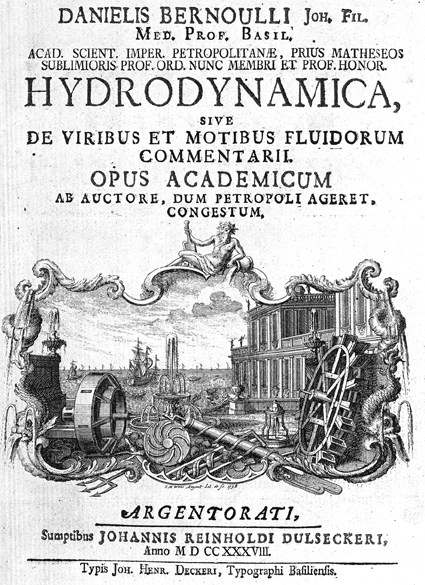
\includegraphics[width=10cm]{bernoulli}
\end{center}

\vfill

\begin{flushright}
  \large{\textsl{Equipe p\'edagogique : \\
      D. Fabre, M. Zagzoule}}
\end{flushright}

\end{titlepage}

%%%%%%%%%%%%%%%%%%%%%%%%%%%%%%%%%%%%%%%%%%%%%%%%%%%%%%%%%%%%%%%%%%%%%%%%%%%%%%%%%%%%%%%%%%%%%%%%%%%
\tableofcontents
%%%%%%%%%%%%%%%%%%%%%%%%%%%%%%%%%%%%%%%%%%%%%%%%%%%%%%%%%%%%%%%%%%%%%%%%%%%%%%%%%%%%%%%%%%%%%%%%%%%


% !TEX root = TD_fluides_part1.tex


%==================================================================================================
\section{Analyse dimensionnelle et similitude}
%==================================================================================================

\subsection{Force de résistance à l'avancement d'un bateau de pêche}

%\section{Résistance à l'avancement d'un pétrolier}

On cherche à déterminer la résistance à l'avancement d'un petit bateau de pêche naviguant dans de l'eau de mer à la vitesse nominale {\color{red} $U = 4 m/s$}.
La longueur du navire est de $L = 10 m$, et sa surface mouillée est de $S = 37,64 m^2$. 

%La masse volumique de l'eau vaut $\rho = 1026 kg/m^3$ pour le navire. La viscosité cinématique de l'eau est $\nu = 1.188 10^{-6} m /s^2$.

\subsubsection{Analyse dimensionnelle}

\begin{enumerate}

\item Listez tous les paramètres physiques pertinents et indépendants ayant une influence sur la force de résistance.

\rep{ Liste des paramètres retenus : $U,L,\rho,g,\nu$ (ou $\mu$),

Paramètres non retenus :
\begin{itemize}
\item $P_0$ (pression de référence "atmosphérique). Justifications possibles : 
$(i)$ expérimentale ; on constate que la traînée ne varie pas en fonction des conditions météo. 
$(ii)$ La force due à la pression est une intégrale de $P$ sur une surface fermée, si on modifie la pression de référence (on remplace $P$ par $P+ \delta_P$ partout) 
  l'intégrale correspondante n'est pas modifiée  (cf. chap. 2 et souvenirs de L2 normalement).
$(iii)$  les équations du mouvement du fluide incompressible (NS) sont invariantes lorsque l'on change $P_0$ en $P_0'$ (cf. chap. 5).

\item $T_0$ : les transferts thermiques ne sont pas pertinents dans ce problème (et de + $T_0$ n'est pas indépendant car pour un fluide incompressible $\rho = \rho(T)$)

\item $\rho_a,\mu_a$ (densité de l'air ; car 1000 fois plus faible que celle de l'eau, la résistance exercée par l'air est donc négligeable)

\item Si on retient $\nu$, $\mu$ n'est pas indépendant (ou inversement).

\item Largeur $\ell$, hauteur $H$, autres dimensions, etc... car si l'on considère une géométrie de bateau donnée, celles-ci sont toutes proportionnelles à la longueur $L$.
(en revanche si l'on considère une famille de géométries dont on souhaite faire varier les caractéristiques, il pourra être pertinent de rajouter des paramètres géométriques comme $\ell/L$ , etc... , mais ici dans la suite on utilisera une maquette géométriquement similaire )

\item  De même la surface mouillée $S$ n'est pas indépendante car $S = \equiv L^2$, le volume non plus.

\item La masse du bateau n'est pas pertinente (elle intervient dans le bilan des forces verticales, mais n'est pas pertinente dans la force horizontale) 

\item De même pour toutes les autres propriétés du bateau (répartition de masse à l'intérieur de celui-ci, etc...) 

\item etc... (l'age du capitaine n'est pas pertinent non plus !)

\end{itemize}

NB les valeurs de $\rho,\nu$,etc... sont données dans le tableau "annexe B".

}



\item En déduire que la résistance à l'avancement peut se mettre sous la forme suivante :

$$ 
R_T = \frac{1}{2} \rho S U^2 \cdot  C_T \left( \frac{U L}{\nu} , \frac{U}{\sqrt{gL}} \right) 
$$  

\rep{
Méthode : on part de la relation $R_T = {\cal F}(U,L,\rho,g,\nu)$. On liste les dimensions physiques des variables retenues.
On met sous forme adimensionnelle sous la forme 
$$
\frac{R_T}{ [M] [L] [T]^{-2} }  = \overline{{\cal F}} \left( \frac{U}{[L] [T]^{-1}},\frac{L}{[L]},\frac{\rho}{[M] [L]^{-3}},\frac{g}{[L] [T]^{-2}},\frac{\nu}{[L]^2 [T]^{-1}} \right)
$$

Le choix le plus judicieux est $[L] = L$, $[M] = \rho L^3$, $[T] = L/U$. On arrive alors à : 
$$
\frac{R_T}{ \rho L^2 U^2 }  = \overline{{\cal F}}\left(1,1,1,\frac{gL }{U^2},\frac{\nu}{L U} \right) 
$$
ce qui est équivalent à la forme recherchée (NB par convention on préfère faire apparaître $S$ plutôt que $L^2$ , c'est équivalent dimensionnellement mais plus pratique à l'usage) .
}




\item Quels nombres adimensionnels classiques reconnaissez-vous là ? quelle est leur interprétation ?

\rep{
On reconnaît les nombres de Froude et Reynolds (s'aider du tableau "annexe A").

Inteprétations : $Re$ = Effets inertiels / Effets visqueux, $Fr$ = effets inertiels /effets gravitationnels). NB : ici les effets gravitationnels se manifestent par la création de vagues. Autre interprétation : $Fr$ =  vitesse du bateau / vitesse des vagues. Analogie avec le nombre de Mach (mais en réalité c'est plus compliqué car les vagues sont des ondes dispersives...).
}   


\item Calculez la valeur de ces deux nombres dans le cas du bateau de pêche en condition réelles.

\rep{  $Fr = 0.4$, $Re = 3.0326 \cdot 10^7$.}  


\subsubsection{Etude de similitude}

On cherche à déterminer la traînée à l'aide d'une expérience en bassin de traction (dans l'eau douce), à l'aide d'une maquette à l'échelle 1/10ème.

\item Est-il possible de faire une expérience en similitude totale (nombres de Froude et de Reynolds identiques dans l'expérience et le navire réel) ? 

\rep{ Similitude de Reynolds => $U_M/U = L/L_M$ ; similitude de Froude (en gravité terrestre, $g=g_M$) => $U_M /U = (L/L_M)^{-1/2}$, impossible d'assurer les deux a moins de faire l'expérience  sur une autre planète !}

\item Quelle doit être la vitesse $U_m$ de la maquette si l'on souhaite respecter la similitude de Reynolds ? Que vaut alors le nombre de Froude de l'expérience ? ce cas vous semble-t-il réaliste ?

	\rep{ $U_m = 40m/s$, $Fr_m = 12.77$, la structure du champ de vagues va être très différente...}


\item Quelle doit être la vitesse $U_m$ de la maquette si l'on souhaite respecter la similitude de Froude ? Que vaut alors le nombre de Reynolds $Re_m$ de l'expérience ?

\rep{ $U_m = 1.26 m/s$ ; $Re_m = 1.2624e6$. } 

\subsubsection{Similitude partielle sous l'hypothèse de Froude} 

 Lorsque $Re \gg 10^{5}$ et $Fr \le 0.4$, l'expérience montre que l'on peut faire l'hypothèse de Froude, qui consiste à supposer que la  résistance à l'avancement se décompose en deux parties données par les expressions suivantes :

$$
C_T(Re, Fr) = {\color{red} C_v} (Re) + C_{w}(Fr) 
$$ 

où $C_v$ est le coefficient de traînée visqueuse, estimé par la loi empirique de Hugues :
$$
C_v(Re) = \frac{0.074}{\left( \log_{10} Re - 2 \right)^2}
$$

et $C_{w}(Fr)$ est la traînée de vagues, qui peut être mesuré en effectuant une expérience en similitude de Froude.

\item  Pour une vitesse d'avance de la maquette correspondant à celle calculée à la question 7, on mesure sur la maquette une résistance à l'avancement 
{\color{red} $R_{T,m}  = 2.228 N$.} 

En déduire la traînée totale exercée sur le navire réel $C_T$, puis la puissance qui doit être fournie par le moteur du bateau.

\rep{Rep : le coefficient de traînée de la maquette vaut 

$C_{T,m} = \frac{ R_{T,m}}{\rho_m S_m U_m^2/2} = 0.074 $. 

La partie visqueuse donnée par la loi empirique vaut $C_{v}(Re_m) = 0.0044$.

En retranchant les deux on déduit $C_w =  0.003$, qui est le même que pour le navire réel.
 
Donc le coefficient de traînée du navire réel vaut $C_T = C_w + C_v(Re) = 0.003 + 0.0025 = 0.0055$, et la traînée totale vaut 
$R_T = 1701 N$.
La puissance correspondante vaut ${\cal P} = R_T U = 6803 W= 9,13$ chevaux-vapeur. 
}


\end{enumerate}



\subsection{Force de traînée sur une automobile}

On cherche à estimer la force de traînée $D$ s'exerçant sur une automobile de longueur $L$ et surface frontale $S$ roulant à la vitesse $V$, à l'aide d'une expérience utilisant une maquette à échelle réduite dans un tunnel hydrodynamique.

\begin{enumerate}
\item Listez et discutez les paramètres physiques pertinents et indépendants dans ce problème.  

%{\em Réponse : $g$ n'est pas pertinent (contribue (faiblement) à la force verticale via la poussée d'Archimède mais pas à la force horizontale), $p_{atm}$ non plus (incompressible car faible Mach), 
%$S$ non plus (proportionnel à $L^2$ pour une géométrie de voiture donnée).
 %Donc $ D= { \cal F} ( V, L, \rho, \nu)$.
%}

\item En utilisant les principes de l'analyse dimensionnelle, montrez que la traînée s'exprime simplement sous la forme suivante :

$$ 
D = \rho S V^2 C_x( Re),  \quad \mbox{ avec } Re = \frac{V L}{\nu}
$$

%{\em Réponse : l'analyse dimensionnelle donne $D/(\rho L^2 V^2) = f(V L/\nu)$, par convention on préfère utiliser la surface de référence $S$ (proportionnelle à $L^2$ pour une géométrie donnée).}


\item Calculez la valeur du nombre de Reynolds, pour une automobile de longueur $L = 4m$ (et surface frontale $S = 1.74 m^2$), roulant à la vitesse $V= 90 km/h$. 

%{\em Réponse : $Re = 1.66 \cdot 10^6$.}

\item Dans l'expérience, la maquette est à l'échelle 1/10 (c.a.d. $L_m = L/10$). La vitesse de l'eau dans le tunnel hydrodynamique est notée $V_m$.

Quelle doit être la valeur de $V_m$ pour assurer la similitude de Reynolds ?

%{\em Réponse : $Re = Re_m$ donc $V_m = \nu_m /L_m Re = 16,6 m/s$}

\item 
Le tunnel hydrodynamique étant réglé à la vitesse $V_m$ précédemment déterminée, 
on mesure à l'aide d'une balance de forces une traînée sur la maquette $D_m = 911 N$.
En déduire le $C_x$, puis la traînée $D$ sur la voiture.

%{\em Réponse : $C_x = 0.38$ ; $D = 260 N$.}

\item En déduire la puissance dissipée par les forces aérodynamiques, puis la puissance qui doit être fournie par le moteur, en supposant que le rendement énergétique global de celui-ci est $\eta = 20 \%$.

%{\em Réponse : $DV = 6.5 kW ; \cal{P} = 65 kW = 87 hp$. ($1 hp$ = 1 cheval-vapeur = $746 W$; unité différente du cheval-fiscal apparaissant sur la carte grise !)
%}

\end{enumerate}
 
 
%{\em Remarque : je ne donne pas les valeurs de la masse volumique et viscosité de l'air et de l'eau, c'est intentionnel, normalement ils devraient les connaitre...}



%\subsection{Traînée d'un bateau}


\subsection{Vitesse d'un animal volant}

On cherche à estimer la vitesse $V$ d'un animal volant (insecte, oiseau ou chauve-souris) en fonction de sa masse $M$.


%\subsubsection{Analyse dimensionnelle}


\begin{enumerate}

\item 

Listez les différents paramètres physiques intervenant dans le problème, et discutez leur pertinence. Montrez qu'il est légitime de supposer que la vitesse est donnée par une loi de la forme 

$$
V = {\cal F}(M,L,\rho,g,\nu).
$$

où $\rho$ est la masse volumique de l'air, $g$ l'accélération de la gravité,
$L$ l'envergure de l'oiseau, $M$ sa masse et $\nu$ la viscosité cinématique de l'air.


%\item Commentez l'hypothèse faite ci-dessus ; quels paramètres physiques 
%n'ont pas été pris en compte et comment justifiez-vous leur omission ?

\item Donnez les dimensions physiques de $V$, $\rho$, $\nu$, $g$, $L$ et $M$.

\item En appliquant les principes de l'analyse dimensionnelle, montrez
que la loi de vitesse peut se mettre sous la forme :

$$
V = \sqrt{gL} \,\, {\cal F} \left(\frac{M}{\rho L^3},\frac{\nu}{\sqrt{g L^3}}\right).
$$

 \item Interprétez physiquement la quantité $M/ (\rho L^3)$. Justifiez pourquoi
on peut supposer en première approximation que cette quantité a la même valeur
pour tous les animaux volants.
 
\item Quelle est l'interprétation physique du nombre sans dimensions $Ga= \frac{\sqrt{g L^3}}{\nu}$ (parfois appelé nombre de Galilée) ?

\item 
Des considérations aérodynamiques permettent de montrer que dans la gamme
$Ga > 10^3$ la structure de l'écoulement est indépendante de la viscosité. Estimez le nombre de Galilée pour les différents animaux volants du tableau ci-dessous.  



\item En déduire que  la vitesse d'un animal volant est proportionnel à
$M^{1/6}$.


\item Application : calculez le rapport $V/M^{1/6}$ pour les différents animaux
détaillés dans le tableau ci-dessous. Commentez les résultats
\begin{center}
\begin{tabular}{|l|l|l|l|}
\hline 
Animal  & Poids & Vitesse & $V/M^{1/6}$ \\
\hline 
Guêpe & $100 mg$ & $20 km/h$ & \\
Colibri & $2.5 g$ & $45 km/h$ & \\
Hirondelle & $17g$ & $60 km/h$ & \\
Aigle & $6kg$ & $160 km/h$ & \\ 
Airbus A300 & $150 T$ & $855 km/h$ & \\
\hline
\end{tabular}
\end{center}

\item En se basant sur l'analyse précédente, à combien estimez vous la vitesse d'une mouette de masse $400g$ ?

 \comment{
\subsubsection{Etude aérodynamique$^*$}

On souhaite retrouver la loi trouvée ci-dessus à partir des équations de l'aérodynamique. On suppose que l'animal a une aile de surface $S$ et vole à l'horizontale.

\item A partir de l'équation de la portance, exprimez la vitesse $V$ 
en fonction de $\rho$, $S$, $m$ et $g$ et $C_L$.

\item Justifiez pourquoi le coefficient $C_L$ est à peu près le même pour
tous les animaux volants.

\item Justifiez pourquoi la surface $S$ est proportionnelle à $M^{2/3}$

\item Retrouvez la loi d'échelle donnant vitesse en fonction de la masse
trouvée à la partie précédente.
}

\end{enumerate}



\comment{
\subsection{Avion et maquette$^*$}


\subsubsection{Avion en vol}

On considère un avion de transport, d'envergure 40 $m$, de longueur 45 $m$, 
de surface de voilure de 260 $m^2$. On suppose qu'il vole à 10 800 $m$ d'altitude à un nombre
de Mach $M_1 = 0.75$.  

Pour l'air on prend les caract\'eristiques suivantes :
  $r = 287.04$ et $\gamma= 1.4$ et 
  
\begin{center}
\begin{tabular}{c |cccc}
  $H$ en m     &  $T$ en   $^\circ K$    & $P$ en $kPa$   &  $\nu$ en $m^2/s$
  \\ \hline  
 10 800       & 218.08    & 23.422     &    $3.8202 \ 10^{-5}$\\
 1 800       & 276.46    & 81.494     &     $1.6869 \ 10^{-5}$
 \end{tabular}
\end{center} 
 

 \begin{enumerate}
 \item Calculer la masse volumique de l'air $\rho_1$, la vitesse du son $a_1$, 
 en déduire la vitesse de l'avion.
 \item Calculer la corde moyenne de l'aile $\ell_1$ et en déduire
 le nombre de Reynolds correspondant. Calculer le nombre de Reynolds $Re_ {L1}$
 basé sur la longueur de l'avion.
 \item Donner l'ordre de grandeur de l'épaisseur de la couche limite sur l'aile 
 à une distance $x_1= 4 \ m$ du  bord d'attaque. 
 
 \item Reprendre les questions précédentes à l'altitude de  1 800 $m$, pour le
 nombre de Mach de $M_1=0.4$.
 
 \item Conclusion
 \end{enumerate} 
 
 
 
\subsubsection{   Maquette de l'avion  au 1/10 ème}
 
   \begin{enumerate}
   \item Donner les grandeurs suivantes $\ell_2$, $L_2$, $S_2$.
    On teste la maquette dans une soufflerie reproduisant une atmosphère
   à $H=10800 \ \  m$. 
   
    \item On cherche une similitude sur le nombre de Reynolds, en déduire la vitesse
   que doit avoir l'air dans la soufflerie. Quelle est alors la valeur du nombre
   de Mach ? En tirer des conséquences sur l'aérodynamique.
   
   \item  On cherche une similitude sur le nombre de Mach, qu'elle est alors
   la valeur du nombre de Reynolds ? En tirer des conséquences sur l'aérodynamique.
   \end{enumerate}
 
 
 
 \subsubsection {   Force de portance}
 Dans les 2 cas précédents,  en déduire la valeur
 de la force de portance $L$, en sachant que le $C_L$ considéré est de $0.175$.
 Conclusions. 
 }

%
%\subsection{Analyse de similitude d'un moteur d'avion à hélice$^*$}
%
%
%On cherche des relations simples, fonctions de nombres sans dimension
%caractéristiques, qui donnent la force de traction $T$ de l'hélice, 
%le couple $Q$ exerçé par l'hélice sur l'arbre moteur
%et la puissance résistante $P_h$ de l'air sur l'hélice. 
%
%
%\begin{enumerate}
%
%\item
%Donner les dimensions et les unités de la force $T$, du diamètre de
%l'hélice $D$, de la fréquence de rotation $n$,
%de la masse volumique $\rho$, de la viscosité cinématique $\nu$, de la vitesse
%de l'avion $V_0$, et de la pression $p$
%
%
%\item En utilisant l'analyse dimensionnelle, montrer que la force de traction
%peut être mise sous la forme suivante :
%
%
%$$
%T =  \rho n^2 D^4 k_T(Re,M,J) ,
%$$
%
%où $Re = V_0 D / \nu$, $M = V_0/c$ avec $c = \sqrt{\gamma P/\rho}$, et 
%$J = V_0 /nD$.
%
%
%\item Interprétez physiquement les paramètres $Re,M$ et $J$.
%
%
%\item Trouver une relation simple du même type avec un coefficient $k_Q$ pour le
%couple $Q$.
%
%\item Ecrire la  puissance sur l'arbre de l'hélice  $P_h$  en fonction
%d'un paramètre sans dimension $C_P$.
%\item La puissance   utile pour la propulsion est 
%$P_u= T V_0$. Calculer le rendement propulsif $\eta_p$  en fonction de nombres sans dimension.
%
%\item Une hélice de diamètre $D=3.4 m$ a les caractéristiques détaillées dans
%la figure 3.
%
%%\begin{center}
%%\begin{tabular}{|c|cccc|}
%%$J$  &  1.06   & 1.19  & 1.34  &  1.44 \\
%%\hline $k_Q$ & 0.0410  & 0.04  & 0.0378  & 0.0355\\
%%\hline $\eta_p$ &  0.76  & 0.80 & 0.84  & 0.86
%%\end{tabular} 
%%\end{center}
%Déterminer la vitesse de l'avion $V_0$ qui lui permet d'absorber une puissance
%de 750 $kW$ à $n=1250  tr/mn$ et à 3660 m d'altitude ($\rho/\rho_0=0.639$) et
%donner la force de propulsion $T$. Pour le calcul numérique $n$ doit être en $tr/s$.
%
%Comparer le rendement de cette hélice à celle d'un propulseur idéal, de même
%surface, et donnant la même propulsion dans les mêmes conditions.
% 
%\end{enumerate}
%  
%   \begin{figure}
%   $$
%  \includegraphics[width = 8cm]{./courbepropulseur.eps}
%  $$
%\caption{   Figure 1 :  Abscisse : $J$, trait continu : $20 \times k_Q$, trait pointillé : $\eta_p$ }
%  \end{figure}
%


% !TEX root = TD_fluides_part1.tex

\section{Hydrostatique}


\setcounter{subsection}{-1}
\subsection{Forces de pression sur un barrage}

%\begin{figure}[H]
%\includegraphics[width=\linewidth]{Biplan.eps}
\input{BarrageTriangulaire.pstex_tm} 
%\end{figure}

On considère un lac dans une vallée de section triangulaire,
d'angle au sommet $2\alpha$.
Le lac est fermé par un barrage de hauteur 
$h$. Le lac est rempli
d'eau de densité constante $\rho$, et sa surface est à la pression 
atmosphérique $P_a$.


\begin{enumerate}

\item Donnez l'expression de la pression $P(z)$ régnant dans le lac, où $z$ est l'altitude 
comptée par rapport à la base du barrage.

\item Calculez la résultante $\vec R$ des forces de pression exercées par l'eau 
et par l'air sur la surface du barrage.

\item Calculez le moment $\vec{\mathcal M}_O$ des forces de pression par
rapport au point $O$.

\item Donnez la position du centre de poussée $F$ des forces de pression.

\end{enumerate}



\subsection{La montgolfière}

On considère une montgolfière, constituée d'un ballon sphérique et de 
rayon $R = 8m$, ouvert à sa base par une ouverture de section négligeable, et d'une nacelle.

On souhaite déterminer la température à laquelle il faut chauffer le gaz intérieur
pour pouvoir voler à l'altitude de $h=1000m$.

\begin{enumerate}

\item En utilisant un modèle d'atmosphère isotherme à tempérarure $T_0 =15^0C = 288K$, donnez les lois $P(z)$ et $\rho(z)$ sachant que la pression au niveau du sol est $P_0 = 1024 hPa$.

\rep{ 
On écrit la loi de l'hydrostatique :
$$
\frac{\partial p}{\partial z } = - \rho g = - \frac{g p}{rT_0 };
$$
Celle-ci s'intègre alors :
$$
\log p - \log p_0  =  - \frac{g z }{ \alpha r T_0}  
$$
Et donc :
$$
p = p_0 e^{-  \frac{g z }{ \alpha r T_0} }
$$
}


\item Donnez la masse volumique 
$\rho_{ext}$ ainsi que la pression $P_{ext,h}$ caractérisant l'air à l'extérieur 
de la montgolfière à l'altitude $h = 1000m$ correspondant à la base du ballon.

\rep{ $ P = 909 hPa$, $\rho = 1.1002 kg/m^3$}

\item
Quelle erreur commet-on en supposant la masse volumique constante à l'échelle du ballon ? 
Montrez que dans cette approximation la pression peut être approximée par une loi affine
de la forme $P_{ext}(z') \approx P_{ext,h}+a z'$ où $z' = z-h_0$ est l'altitude comptée à partir
de la base du ballon.

\rep{ 
En remplaçant $z=1000m$ par $z=10016m$ (2x le rayon) on trouve une variation de masse volumique de 0,3 $\%$.
On peut supposer $\rho \approx \rho_h$ et $P_{ext} = p_h - \rho_h g z'$.
}
  
\item Le ballon est rempli d'air de masse volumique $\rho_{int}$ supposée uniforme.
Donnez la loi de pression $P_{int}(z')$ à l'intérieur du ballon.

\rep{ 
 $P_{int} = P_{ext,h} - \rho_{int} g z'$.
}

\item Calculez la résultante des efforts exercés par l'air sur le ballon.

\rep{Poser l'intégrale en coordonnés sphériques...}

\item Retrouvez le résultat précédent à l'aide du théorème d'Archimède.

\rep{
$ 
F = ( \rho_{ext} - \rho_{int} ) m g 
$
}

\item Application : calculez la valeur de $\rho_{int}$ nécessaire pour 
maintenir la montgolfière en équilibre à l'altitude 1000m, considérant que 
sa masse totale est $m=600kg$. En déduire la température $T_{int}$
mesurée à la base du ballon.

\rep{ On trouve $\rho_{int} = \rho_{ext} - m/V = 0.821 kg/m^3$.
La température correspondante est alors $T_{int} = 397 K = 124 K$.
}



\end{enumerate} 



\subsection{Modèle d'atmosphère normalisée}

Le {\em modèle d'atmosphère normalisée }  ( \verb| http://fr.wikipedia.org/wiki/Atmosphère_normalisée | )
est un modèle adopté internationalement qui découpe l'atmosphère en sept couches successives
dans lesquelles la température est donnée par une loi affine de la forme 
$$T(z) = T_0 ( 1 - \alpha z)$$. On considère ici uniquement la couche inférieure appelée troposphère ($0<z<11km$) dans laquelle
les paramètres de cette loi sont  $\alpha = 22.6 \cdot 10^{-6} m^{-1}$ et $T_0 = 288 K$.  

Donnez les loi $P(z)$ et $\rho(z)$ correspondantes, sachant que la pression au niveau du sol
est $P_0 = 1013 hPa$.

\rep{ 
On écrit la loi de l'hydrostatique :
$$
\frac{\partial p}{\partial z } = - \rho g = - \frac{g p}{rT_0 ( 1 - \alpha z ) };
$$
Celle-ci s'intègre alors :
$$\log p - \log p_0  =  \frac{g}{ \alpha r T_0}   \log (1- \alpha z) 
$$
Et donc :
$$
p = p_0 {\left( 1 - \alpha z \right)}^{\frac{g}{ \alpha r T_0} }  
$$
}

Répondre à la dernière question de l'exercice précédent dans le cas de ce modèle d'atmosphère amélioré.
  
\subsection{Envasement d'une barge}


%\begin{figure}[H]
%\includegraphics[width=\linewidth]{Biplan.eps}
\input{BargeVase.pstex_tm} 
%\end{figure}
  
On considère une barge de section carrée, de largeur $b=10m$ de hauteur 
$h=1m$,  et de masse $M = 75 t$. 
La barge flotte dans de l'eau de densité $\rho_e=1000kg m^{-3}$.
A marrée haute la hauteur d'eau est $H > h$.
  
  
\begin{enumerate}

\item Calculez le tirant d'eau de la barge à marée haute.


\item A marée basse la hauteur d'eau est de $H =25cm$, et la barge
s'enfonce dans la vase, que l'on considère comme un fluide de masse volumique
$\rho_v = 2 \rho_e$.
Calculez la profondeur d'envasement $e$.

%\item Calculez l'allègement qu'il faudrait faire subir à la barge pour éviter
%son envasement.


\end{enumerate}  


\subsection{Lois de pression et de température dans l'océan}

On cherche à estimer les lois de pression $P(z)$ et de 
masse volumique $\rho(z)$ dans l'océan en fonction de la profondeur $z$.
Les altitudes $z$ sont comptées vers le bas à partir de la surface
de l'océan, et la pression au niveau de la mer est $P_0 = 1,013 Bars$, en utilisant les modèles suivants:

\begin{itemize}

\item La couche superficielle, qui s'étend jusqu'à environ 500 mètres de 
profondeur, est appelée thermocline. Dans cette couche la température
varie entre $T = 25^o C$ (en surface) et $T = 1.5^o C$ (à la base de la
thermocline). On suppose pour simplifier que la salinité est constante ($S = 35g/kg$).

On supposera que dans la thermocline la compressibilité est négligeable, de sorte que 
la masse volumique dépend seulement de la température, et est donnée par la relation 
simplifiée suivante (issue de l'équation d'état officielle IES80, avec $T$ en $^o C$, $\rho$ en $kg/m^3$ cf. Formulaire A3) :

$
\rho = 1028.15 - 0.05403 \times T - 0.006762\times  T^2 +7.955\cdot 10^{-5} \times T^3 - 9.3152 \cdot 10^{-7} \times T^4
+ 6.5363  \cdot 10^{-9}  \times T^5.
$


%$\rho$ évolue notablement, principalement 
%sous l'effet de variations de température et de salinité.
%Plus précisément, la masse volumique passe de $\rho_0 = 1023 kg m^{-3}$
%en surface $(z=0)$, à la valeur $\rho_1 = 1030 kg m^{-3}$ à la profondeur
%$z_1 = 500 m$. 
%A la base de celle-ci 
%la température est $T_1 = 1.5 ^o C$.


\item Dans les couches plus profondes,  à cause de la compressibilité de l'eau de mer, la masse volumique et la température varient (faiblement) en fonction de la pression. On supposera que dans les couches profondes les coefficients
thermodynamiques et thermoélastiques sont constants, et ont les valeurs suivantes :

$
\chi_s = 4.6 \cdot 10^{-10} Pa^{-1} ; \quad 
\alpha_p = 8 \cdot 10^{-5} K^{-1} ; \quad 
c_p = 4000 J \cdot K^{-1} \cdot kg^{-1}.  
$

%où $\rho_1$ et $P_1$ sont les valeurs à la base de la thermocline, 
%et $K$ est un "coefficient d'élasticité", 
%supposé constant, qui vaut :

%$$
%K = 23000 Bars.
%$$

%$$
%\chi = \frac{1}{\rho} 
%{\left(\frac{\partial \rho}{\partial p}\right)}_{T,S} = 4,5 \times 10^{-10} 
%Pa^{-1}.
%$$




\end{itemize}

\begin{enumerate}

\item Donnez la masse volumique en surface ($\rho_0$) et à la base de 
la thermocline ($\rho_1$). En déduire la loi de masse volumique $\rho(z)$  
dans la thermocline, en supposant qu'elle varie linéairement avec la profondeur.

\item  Déduisez-en la loi de pression $P(z)$ dans la thermocline.
Donnez en particulier la pression $P_1$ à la base de la thermocline. 


\item Dans les couches profondes, la masse volumique peut s'exprimer 
en bonne approximation par l'équation linéaire suivante :
$$
\rho = \rho_1 \left( 1 + \chi_s (P-P_1) \right).
$$ 
Donnez les lois de pression $P(z)$  et de masse volumique dans les 
couches profondes de l'océan ($z>z_1$). 
Donnez une approximation polynômiale de ces lois sous la forme
 $P(z) = P_1 + a (z-z_1)+ b (z-z_1)^2$, et $\rho(z) = \rho_1 + c (z-z_1)$.

\item 
Démontrez la relation suivante entre les coefficients thermodynamiques : 
$$
\epsilon_s = \frac{1}{T}
{\left(\frac{\partial T}{\partial  P}\right)}_{s} = \frac{\alpha_p}{\rho c_p}
$$

\item Déduisez-en la loi de température $T(z)$ dans les couches profondes $(z>z_1)$.


\item Application. La fosse océanique la plus profonde sur terre est située dans le 
Pacifique, au large de l'archipel des Mariannes, 
et atteint la profondeur $z=11000 m$. 
Donnez la pression (en bars), la masse volumique et la température 
reignant à cette profondeur.

%Quelle erreur aurait été commise sur la pression calculée précédemment 
%si on avait supposé la masse volumique de l'eau constante, 
%de valeur $\rho = 1030 kg m^{-3}$ ?

%\item Montrez que dans les couches profondes, 
%la loi de masse volumique calculée précédemment peut être remplacée
%en première approximation par une loi linéaire 
%de la forme $\rho = \rho_1 + A(z-z_1)$, et la loi de pression par une loi
%quadratique de la forme $P = P_1+B(z-z_1)+C(z-z_1)^2$.
%Donnez l'erreur commise en faisant cette approximation pour la profondeur 
%de la fosse des Mariannes.
\end{enumerate}

%\clearpage





\Archives{

\centerline{\fbox{\textbf{\Large Thème 1 : Statique des fluides}}}

\vspace{.5cm}


%%%%%%%%%%%%%%%%%%%%%%%%%%%%%%%%%%%%%%%%%%%%%%%%%%%%%%%%%%%%%%%%%%%%%%%%%%%%%%%
\subsection{Modèles d'atmosphère}
%%%%%%%%%%%%%%%%%%%%%%%%%%%%%%%%%%%%%%%%%%%%%%%%%%%%%%%%%%%%%%%%%%%%%%%%%%%%%%%

L'atmosphère est constitué d'air, considéré comme un gaz parfait avec $ r = 287 J/K/kg$.
Au sol ($z=0$), on a une temp\'erature $T_0 = 288$ K et une pression
$P_0 = 1.013 \; 10^5$ Pa. 

D\'eterminer la loi de pression $P(z)$ en fonction de l'altitude $z$
pour les trois modèles suivants :
\begin{enumerate}
\item
Atmosphère isotherme~: $T(z) = T_0$.
\item
Atmosphère adiabatique : pression et masse volumique sont reliés par
une relation de la forme $p \rho ^{-\gamma} = cte$.

\item 
Atmosphère "standart", c'est à dire dont la température varie selon la loi 
$T(z) = T_0 (1 - \alpha z)$ avec $\alpha = 22.6 \; 10^{-6}$m$^{-1}$ pour $0<z<11 km$,
et est constante, avec la valeur $T = T_1 = 216,4 K$, au delà de cette altitude
(modèle adopté au cours d'une conférence internationale d'aéronautique en 1910)

\end{enumerate}
Pour chaque cas, on calculera la pression au sommet de l'Everest ($z = 8848 m$), 
à l'altitude de vol du Concorde ($z=20km$).




%%%%%%%%%%%%%%%%%%%%%%%%%%%%%%%%%%%%%%%%%%%%%%%%%%%%%%%%%%%%%%%%%%%%%%%%%%%%%%%
\subsection{Distribution de pression dans les oc\'eans}
%%%%%%%%%%%%%%%%%%%%%%%%%%%%%%%%%%%%%%%%%%%%%%%%%%%%%%%%%%%%%%%%%%%%%%%%%%%%%%%

L'eau de mer a une concentration en sel et une temp\'erature 
qui varient suivant la profondeur,
ce qui conduit \`a une masse volumique non homog\`ene dans le fluide
(\textsl{stratification}) que l'on peut mod\'eliser par la loi lin\'eaire~:
$\rho (z) = \rho_0 + \alpha z$, o\`u $z>0$ d\'esigne la profondeur.
$\rho_0 = 1025$ kg/m$^{\mbox{\footnotesize 3}}$ est la masse volumique
de l'eau de mer en surface et $\alpha \sim 0.003$ est une mesure
du gradient de densit\'e.
Cette loi est valable jusqu'\`a une profondeur $z_1= 1000$~m
(\textsl{pycnocline}).
Au-del\`a, la masse volumique est constante, \'egale \`a
$\rho_1 = 1028$ kg/m$^{\mbox{\footnotesize 3}}$

\begin{enumerate}
\item
Calculer la distribution de pression hydrostatique $p(z)$ 
dans les couches pycnoclines en fonction
de la masse volumique au niveau de la surface libre $\rho_0$,
de l'acc\'el\'eration de la pesanteur $g$, 
du param\`etre $\alpha$ et de $P_a$, pression atmosph\'erique au niveau de
la surface libre $z=0$ (figure~\ref{fig:distrib}a).
Estimer l'influence du gradient de masse volumique sur le r\'esultat
obtenu et commenter.
\item
Puis calculer la distribution de pression dans les couches inf\'erieures
($z>z_1$) en fonction de $P_a$, $\rho_1$, $g$, $\alpha$ et $z_1$.
\end{enumerate}

%\begin{figure}[hbt]
%\begin{center}
%\input{../FIGURES/stratif.pstex_t} \qquad \input{../FIGURES/miscib.pstex_t}
%\end{center}
%\caption{(a) Distribution de masse volumique dans les oc\'eans.
%(b) R\'ecipient rempli de deux fluides non miscibles en \'equilibre statique
%dans le champ de pesanteur.}
%\label{fig:distrib}
%\end{figure}


%%%%%%%%%%%%%%%%%%%%%%%%%%%%%%%%%%%%%%%%%%%%%%%%%%%%%%%%%%%%%%%%%%%%%%%%%%%%%%%
\subsection{Transmission de la pression}
%%%%%%%%%%%%%%%%%%%%%%%%%%%%%%%%%%%%%%%%%%%%%%%%%%%%%%%%%%%%%%%%%%%%%%%%%%%%%%%


\begin{figure}[htb]
\begin{center}
\input{../FIGURES/cornue.pstex_t} \quad \input{../FIGURES/levage.pstex_t}
\end{center}
%\caption{}
%\label{fig:transmission}
\end{figure}

\begin{enumerate}
\item
Soit le r\'ecipient de la figure (a), rempli jusqu'en $z=h$ d'un liquide de
masse volumique $\rho$.
Calculer la force exerc\'ee par le liquide sur le fond du r\'ecipient,
de surface $S$.
Commenter.
\item
On souhaite soulever une charge de masse $m$ \`a l'aide du dispositif de
la figure (b).
Pour cela, on applique une force $F$ sur un piston de section $s \ll S$
et de masse n\'egligeable.
En supposant $h \sim H$, calculer la force $F$ n\'ecessaire pour maintenir
le syst\`eme hydraulique \`a l'\'equilibre.
Commenter.
A.N. $m$=1000 kg, $S$ = 1 m$^{\mbox{\footnotesize 2}}$, 
$s$ = 1 cm$^{\mbox{\footnotesize 2}}$.
\end{enumerate}


%%%%%%%%%%%%%%%%%%%%%%%%%%%%%%%%%%%%%%%%%%%%%%%%%%%%%%%%%%%%%%%%%%%%%%%%%%%%%%%
\subsection{Basculement d'une digue {\small \it (Partiel 2004)}}
%%%%%%%%%%%%%%%%%%%%%%%%%%%%%%%%%%%%%%%%%%%%%%%%%%%%%%%%%%%%%%%%%%%%%%%%%%%%%%%



\noindent Une digue en b\'eton, de masse volumique $\rho_b$, retient
de l'eau de masse volumique $\rho_e$. La digue est soumise \`a des
forces de diff\'erentes natures : les forces de pression d\^ues \`a
l'eau et \`a l'atmosph\`ere, son propre poids $\vec{P}$ et la force de
r\'eaction $\vec{R}$ du sol.

\noindent Localement, les forces de pression exerc\'ees par l'eau en
un point $M(y,z)$ de la digue sont not\'ees $\mathrm{d}\vec{F}$. Leur
r\'esultante, not\'ee $\vec{F}$, a pour point d'application $C$,
d\'efini par $\overrightarrow{OC} \wedge \vec{F} = \int \!\!\! \int_S
\overrightarrow{OM} \wedge \mathrm{d}\vec{F}$. On admet que $C$
appartient au plan vertical $x = -L/2$ (face en contact avec l'eau).

\noindent On cherche \`a d\'eterminer sous quelles conditions la digue
peut basculer.

\begin{enumerate}
\item D\'eterminer la r\'esultante $\vec{F}$ des forces de pression
  ainsi que la coordonn\'ee $z_C$ de son point d'application.
\item D\'eterminer le poids $\vec{P}$ de la digue ainsi que la
  coordonn\'ee $x_G$ de son centre de gravit\'e $G$.
\item On pose $\vec{F} = F \vec{e_x}$, $\vec{P} = -P \vec{e_z}$ et
  $\vec{R} = -R_x \vec{e_x} + R_z \vec{e_z}$. Le point d'application
  de $\vec{R}$ est not\'e $N$ et $x_N$ la coordonn\'ee de $N$ suivant
  $\vec{e_x}$.
  \begin{enumerate}
  \item \'Ecrire les conditions d'\'equilibre de la digue
    (r\'esultantes et moments).
  \item En d\'eduire les expressions de $R_x$ et $R_z$ en fonction de
    $F$ et de $P$.
  \item Donner l'expression de $x_N$ en fonction de $F$ et $R_z$.
  \end{enumerate}
\item Afin d'\'eviter le basculement de la digue par rapport au point
  B sous la pression de l'eau, on exige par s\'ecurit\'e que $x_N < L
  / 6$ pour $h_e = h$. Quelle relation doit alors v\'erifier le
  rapport des masses volumiques $\beta = \rho_b / \rho_e$ ?
\end{enumerate}
\begin{figure}[htbp]
  \centering
  \begin{tabular}{cc}
    \begin{picture}(8,4)(0,0)
    \put(0,4){(a)}
    \put(0,0){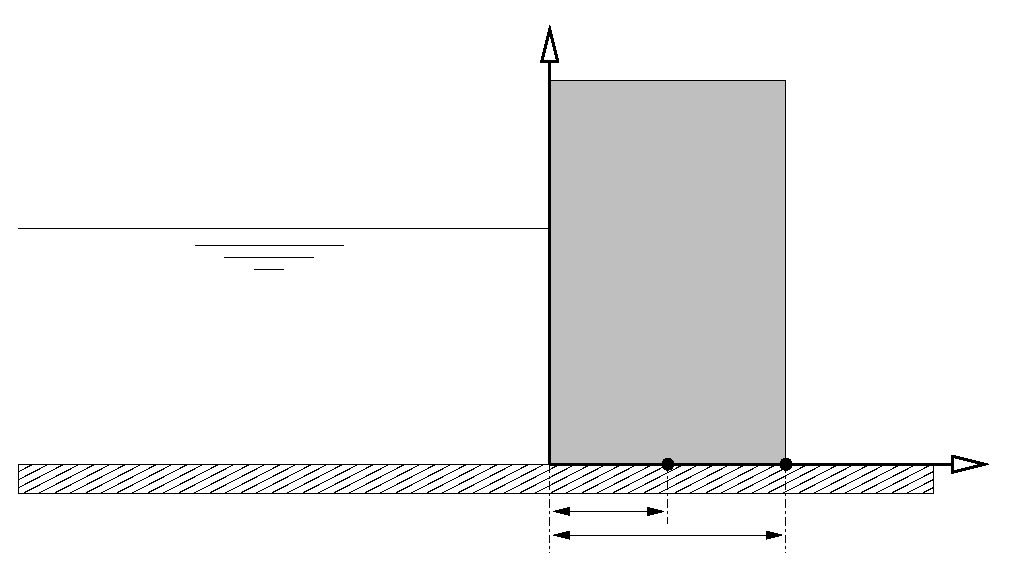
\includegraphics[width=8cm]{digue_coupe.eps}}
    \put(4,3.8){\small $h$}
    \put(4.5,4.2){\small $\vec{e}_z$}
    \put(3.9,2.8){\small $h_e$}
    \put(5.1,0.9){\small $O$}
    \put(4.5,0.4){\small $L/2$}
    \put(5.1,-0.2){\small $L$}
    \put(6.4,0.9){\small $B$}
    \put(7.5,1.0){\small $\vec{e}_x$}
    \end{picture} &
    \begin{picture}(4,4)(-0.5,0)
    \put(0.5,0.5){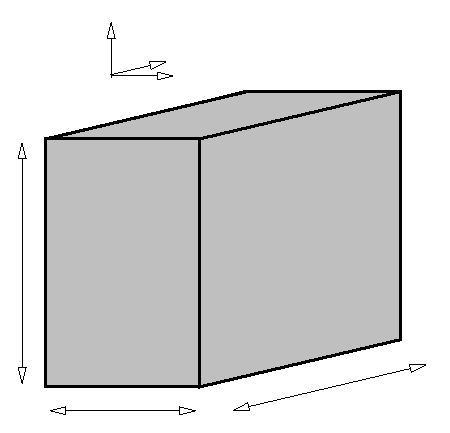
\includegraphics[width=4cm]{digue_perspective.eps}}
    \put(-0.5,4){(b)}
    \put(1.8,3.55){\tiny $\vec{e}_x$}
    \put(1.9,4.){\tiny $\vec{e}_y$}
    \put(1.1,4.2){\tiny $\vec{e}_z$}
    \put(0.2,1.9){\small $h$}
    \put(1.3,0.1){\small $L$}
    \put(3.6,0.4){\small $l$}
    \end{picture}
  \end{tabular}
  \caption{(a) Digue vue en coupe dans le plan $(\vec{e}_x,
    \vec{z})$. (b) Digue vue en perspective.}
  \label{fig:digue}
\end{figure}

%%%%%%%%%%%%%%%%%%%%%%%%%%%%%%%%%%%%%%%%%%%%%%%%%%%%%%%%%%%%%%%%%%%%%%%%%%%%%%%
\subsection{Cylindre immerg\'e dans deux fluides non miscibles}
%%%%%%%%%%%%%%%%%%%%%%%%%%%%%%%%%%%%%%%%%%%%%%%%%%%%%%%%%%%%%%%%%%%%%%%%%%%%%%%

\noindent
Un solide assimilable \`a un cylindre de section $S$ et de hauteur $H$,
de masse volumique $\rho_c$ est immerg\'e dans un r\'ecipient contenant
deux liquides non miscibles homog\`enes de masses volumiques constantes
$\rho_1$ et $\rho_2$.
On rep\`ere la position du cylindre par l'altitude $z$ de sa partie
sup\'erieure par rapport \`a l'interface (figure~\ref{fig:glacon}a).

Ecrire l'\'equation permettant de d\'eterminer la position d'\'equilibre $z_0$
du cylindre \`a l'interface entre les deux fluides
et discuter l'existence d'une position d'\'equilibre et sa stabilit\'e.

\begin{figure}[htb]
\begin{center}
\input{../FIGURES/cyl-misc.pstex_t} \qquad \input{../FIGURES/glacon.pstex_t}
\end{center}
\caption{Cylindre en \'equilibre \`a l'interface entre deux fluides non
miscibles (a). Gla\c{c}on flottant \`a la surface d'un verre d'eau (b).}
\label{fig:glacon}
\end{figure}

%%%%%%%%%%%%%%%%%%%%%%%%%%%%%%%%%%%%%%%%%%%%%%%%%%%%%%%%%%%%%%%%%%%%%%%%%%%%%%%
\subsection{Fonte d'un gla\c{c}on}
%%%%%%%%%%%%%%%%%%%%%%%%%%%%%%%%%%%%%%%%%%%%%%%%%%%%%%%%%%%%%%%%%%%%%%%%%%%%%%%

Un gla\c{c}on est en \'equilibre \`a la surface d'un verre d'eau 
compl\`etement rempli (figure~\ref{fig:glacon}b).
En utilisant le principe de conservation de la masse et le th\'eor\`eme
d'Archim\`ede, d\'eterminer le niveau d'eau dans le verre une fois
le gla\c{c}on fondu.
Le verre d\'eborde-t'il ?


%%%%%%%%%%%%%%%%%%%%%%%%%%%%%%%%%%%%%%%%%%%%%%%%%%%%%%%%%%%%%%%%%%%%%%%%%%%%%%%
\subsection{Stabilit\'e d'un bateau}
%%%%%%%%%%%%%%%%%%%%%%%%%%%%%%%%%%%%%%%%%%%%%%%%%%%%%%%%%%%%%%%%%%%%%%%%%%%%%%%



Lorsqu'un bateau est \'ecart\'e de sa position d'\'equilibre, il subit
de la part du poids et de la pouss\'ee d'Archim\`ede un couple qui
peut soit le redresser et le ramener \`a sa position d'\'equilibre
(que l'on qualifie alors de stable), soit le faire chavirer
(\'equilibre instable).
\begin{figure}[htbp]
  \centering
  \begin{tabular}{cc}
    \begin{picture}(6,3)(0,0)
    \put(0,3){(a)}
    \put(0,0){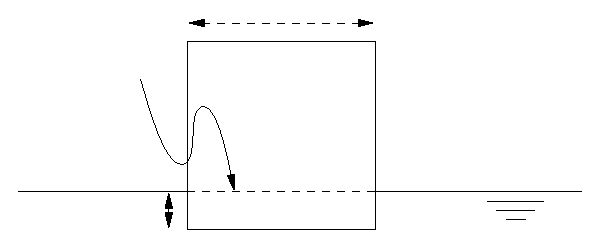
\includegraphics[width=6cm]{stable_equilibre.eps}}
    \put(1.2,0.1){$h$}
    \put(0.0,2.1){\small \textit{Ligne de}}
    \put(0.0,1.7){\small \textit{flottaison}}
    \put(2.6,2.5){$L$}
    \end{picture} &
    \begin{picture}(6,3)(0,0.15)
    \put(0,3.15){(b)}
    \put(0,0){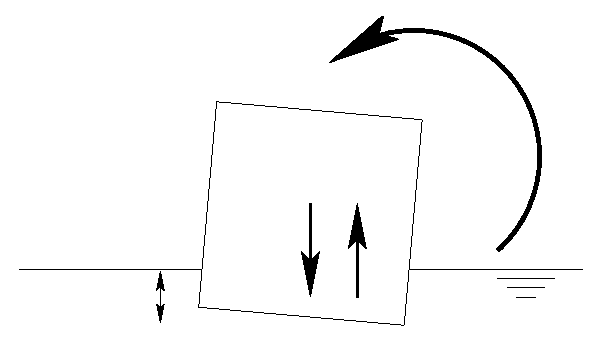
\includegraphics[width=5.5cm]{stable_gitee.eps}}
    \put(0.9,0.2){$h$}
    \put(2.2,0.5){$\vec{P}$}
    \put(3.3,0.5){$\vec{R}$}
    \put(4.0,3){\textit{Couple de}}
    \put(4.8,2.5){\textit{redressement}}
    \end{picture} \\
    \begin{picture}(6,4)(0,0)
    \put(0,3){(c)}
    \put(0,0){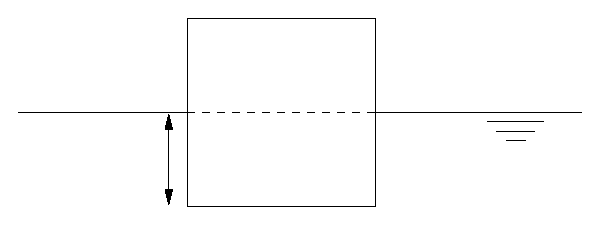
\includegraphics[width=6cm]{instable_equilibre.eps}}
    \put(1.0,0.3){$h$}
    \end{picture} &
    \begin{picture}(6,4)(0,0.25)
    \put(0,3.25){(d)}
    \put(0,0){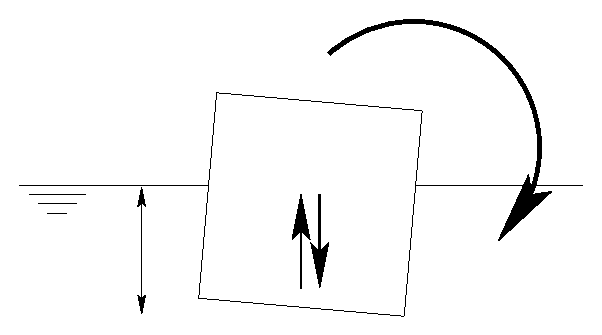
\includegraphics[width=5.5cm]{instable_gitee.eps}}
    \put(0.7,0.4){$h$}
    \put(2.2,0.5){$\vec{R}$}
    \put(3.1,0.5){$\vec{P}$}
    \put(4.0,3){\textit{Couple de}}
    \put(4.8,2.5){\textit{chavirement}}
    \end{picture}
  \end{tabular}
  \caption{(a) Configuration d'\'equilibre stable. Une fois git\'e (b), le bateau subit de la part du poids et de la pouss\'ee d'Archim\`ede un couple qui le ram\`ene \`a sa position d'\'equilibre. (c) Configuration instable. Une fois \'ecart\'e de sa position d'\'equilibre, l'action du poids et de la force d'Archim\`ede tend \`a faire chavirer le bateau.}
  \label{fig:equilibre}
\end{figure}

Dans cet exercice, on s'int\'eresse \`a la stabilit\'e d'un bateau
id\'ealis\'e sous la forme d'un carr\'e de densit\'e uniforme $\rho_b$. Le bateau d'ar\^ete $L$ est
immerg\'e sur une hauteur $h$, que l'on appelle le tirant d'eau. Le
rapport entre la masse volumique du bateau $\rho_b$ et celle du fluide
$\rho_f$ sera not\'ee $\beta$.

Dans un premier temps, la stabilit\'e de la position o\`u une ar\^ete
est horizontale est envisag\'ee.

\begin{enumerate}
\item Ecrire la condition d'\'equilibre du bateau et en d\'eduire une
  relation liant $\beta$, $h$ et $L$.
\item Calculer la position du centre de car\`ene $C$ et du centre de
  gravit\'e $G$.
\item Le bateau est tr\`es l\'eg\`erement git\'e d'un angle $\alpha$
  ($\alpha \ll 1$). Donner la position du nouveau centre de car\`ene $C'$.
\end{enumerate}
Pour \'etudier la stabilit\'e d'un \'equilibre, il est utile
d'introduire un point fictif appel\'e \textbf{m\'etacentre}, situ\'e
\`a l'intersection de $(CG)$ et d'une verticale passant par $C'$.

\begin{enumerate}
\setcounter{enumi}{3}
\item Calculer la distance $CM$ et v\'erifier qu'elle est bien \'egale
  \`a $I/W$, avec $I = \int_\mathrm{flottaison} x^2 \mathrm{d}S$ et
  $W$ est le volume de fluide d\'eplac\'e, encore appel\'e \textit{d\'eplacement}.
\item Discuter de la stabilit\'e du bateau en fonction de la position
  relative de $G$ et $M$.
\item En d\'eduire les valeurs de $\beta$ pour lesquelles cet
  \'equilibre est stable.

\item Refaire l'étude précédente dans le cas où le bateau
pr\'esente une diagonale horizontale.

 
\end{enumerate}
 \vspace{3cm}
\begin{figure}[htbp]
% 
  \centering
  \begin{picture}(6,5)(0,0)
  \put(0,0.5){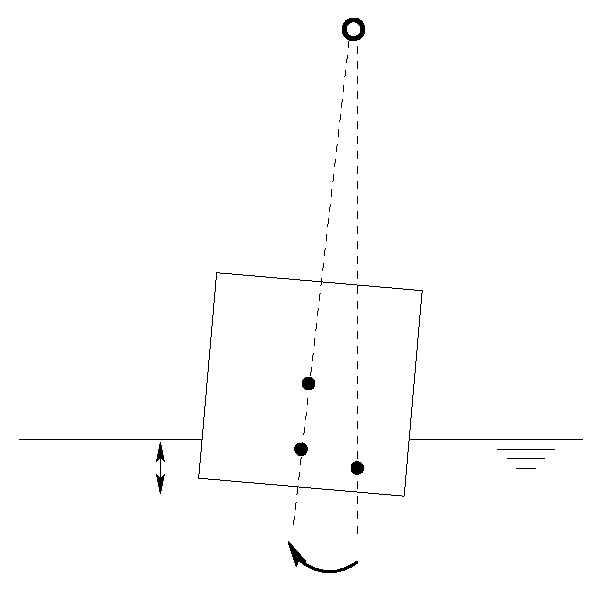
\includegraphics[width=6cm]{metacentre.eps}}
  \put(1.0,1.5){$h$}
  \put(2.5,1.7){$C$}
  \put(2.6,2.5){$G$}
  \put(3.7,1.7){$C'$}
  \put(3.1,0.2){$\alpha$}
  \put(2.9,6.2){$M$}
  \end{picture}
  \caption{Construction du m\'etacentre. Le bateau est \'ecart\'e de sa position d'\'equilibre d'un angle de g\^ite $\alpha$. Le m\'etacentre $M$ est situ\'e \`a l'intersection de $(CG)$ et de la verticale passant par $C'$.}
  \label{fig:metacentre}
\end{figure}

%On s'int\'eresse maintenant \`a la stabilit\'e de l'\'equilibre du
%bateau lorsque celui-ci 
%\begin{figure}[htbp]
%  \centering
%  \begin{picture}(6,3)(0,0)
%    \put(0,0){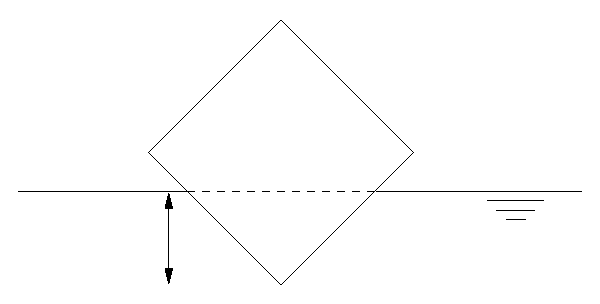
\includegraphics[width=6cm]{diagonale.eps}}
%    \put(1.1,0.4){$h$}
%  \end{picture}
%  \caption{Configuration o\`u le bateau pr\'esente une diagonale horizontale.}
%  \label{fig:diagonale}
%\end{figure}






\comment{
\begin{enumerate}
\setcounter{enumi}{6}
\item Ecrire \`a nouveau les conditions d'\'equilibre et trouver une
  relation connectant $\beta$, $h$ et $L$.
\item Trouver la position du centre de car\`ene et du centre de
  gravit\'e.
\item Donner la position du m\'etacentre. On pourra utiliser la
  relation $CM = I/W$.
\item En d\'eduire un ou plusieurs intervalles de $\beta$ pour lequel
  (lesquels) cet \'equilibre est stable.
\item Rasssemblez les r\'esultats des questions 6 et 10. Que se passe-t'il pour les valeurs de $\beta$ ne correspondant pas \`a ces questions ?
\end{enumerate}


 
%%%%%%%%%%%%%%%%%%%%%%%%%%%%%%%%%%%%%%%%%%%%%%%%%%%%%%%%%%%%%%%%%%%%%%%%%%%%%%%
\subsection{Force d'adh\'esion d'une goutte}
%%%%%%%%%%%%%%%%%%%%%%%%%%%%%%%%%%%%%%%%%%%%%%%%%%%%%%%%%%%%%%%%%%%%%%%%%%%%%%%

\noindent Deux surfaces mouill\'ees peuvent coller tr\`es fortement
ensemble si le liquide les mouille avec un angle de contact $\theta_c$
inf\'erieur \`a un angle seuil $\theta_s$.

\noindent On \'ecrase une grosse goutte entre deux plaques distantes
de $H$. La goutte \'ecras\'ee forme ce que l'on appelle un
\textit{pont capillaire}, illustr\'e sur la figure~\ref{fig:goutte}.
Notons $R$ son rayon et $A \sim \pi R^2$ sa surface. La loi de Laplace
\begin{equation}
  \label{eq:laplace}
  \Delta p = \gamma \left( \frac{1}{R} + \frac{1}{R'} \right)
\end{equation}
va nous permettre d'\'evaluer la saut de pression \`a l'interface.

\begin{enumerate}
\item D\'eterminer la courbure $C = 1/R + 1/R'$ de la surface au
  niveau du point $M$.
\item En d\'eduire le saut de pression \`a l'interface en fonction de
  la tension superficielle $\gamma$, du rayon $R$, de l'angle de
  contact $\theta_c$ et de l'\'ecartement $H$ des plaques. Donner une
  estimation de ce saut dans la limite o\`u $R \gg H$. Dans toute la
  suite, on se place dans cette limite.
\item Donner la valeur limite $\theta_s$ de l'angle de contact \`a ne
  pas d\'epasser pour que cette force soit attractive.
\item Application num\'erique : \\ En prenant $R = 1\,\mathrm{cm}$, $H = 5\,
  \mu\mathrm{m}$, $\theta_c = 0$ et $\gamma~=~72\,\mathrm{mN/m}$ (tension superficielle de l'eau), donner une estimation de la
  d\'epression dans la goutte, ainsi que de la force d'adh\'esion
  r\'esultante. 

  \noindent On accroche maintenant un r\'ecipient \`a la plaque
  inf\'erieure. Quel volume d'eau la plaque peut-elle supporter
  gr\^ace \`a la force d'adh\'esion cr\'e\'ee par cette goutte ?
\end{enumerate}
\begin{figure}[htbp]
  \centering
  \begin{tabular}{c}
    \begin{picture}(8,4)(0,0)
    \put(0,0){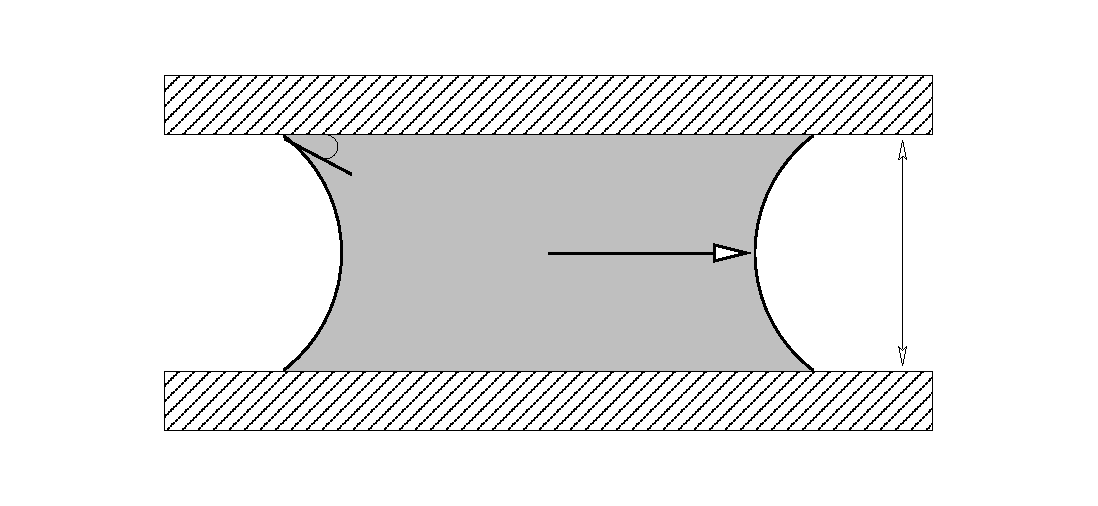
\includegraphics[width=8cm]{goutte.eps}}
    \put(2.6,2.3){\small $\theta_c$}
    \put(5.6,1.7){\small $M$}
    \put(4.6,1.9){\small $R$}
    \put(6.8,1.7){\small $H$}
    \end{picture} 
  \end{tabular}
  \caption{Goutte coinc\'ee entre deux plaques et formant un pont capillaire.}
  \label{fig:goutte}
\end{figure}


%%%%%%%%%%%%%%%%%%%%%%%%%%%%%%%%%%%%%%%%%%%%%%%%%%%%%%%%%%%%%%%%%%%%%%%%%%%%%%%
\subsection{Pression dans deux fluides non miscibles}
%%%%%%%%%%%%%%%%%%%%%%%%%%%%%%%%%%%%%%%%%%%%%%%%%%%%%%%%%%%%%%%%%%%%%%%%%%%%%%%

Un r\'ecipient contient deux fluides non miscibles (par exemple de l'huile
et de l'eau) de masses volumiques respectives $\rho_1$ et $\rho_2$,
constantes (figure~\ref{fig:distrib}b).
La pression atmosph\'erique r\'egnant \`a l'ext\'erieur, not\'ee $P_a$,
est suppos\'ee constante. 
\begin{enumerate}
\item
D\'eterminer la distribution de pression $p_1(z)$ dans le liquide 1
($z\in[h, H]$) en fonction de $\rho_1$, $H$, $g$ et $P_a$.
\item
D\'eterminer la distribution de pression $p_2(z)$ dans le liquide 2
($z\in[0, h]$)
en fonction de $\rho_1$, $\rho_2$, $h$, $g$, $P_a$ et $e=H-h$.
\item
Calculer la r\'esultante des forces de pression exerc\'ees par les fluides
(air et liquides) sur le fond du r\'ecipient, de surface $S$.
Interpr\'eter le r\'esultat obtenu.
\end{enumerate}


%%%%%%%%%%%%%%%%%%%%%%%%%%%%%%%%%%%%%%%%%%%%%%%%%%%%%%%%%%%%%%%%%%%%%%%%%%%%%%%
\subsection{Efforts de pression sur un barrage}
%%%%%%%%%%%%%%%%%%%%%%%%%%%%%%%%%%%%%%%%%%%%%%%%%%%%%%%%%%%%%%%%%%%%%%%%%%%%%%%

\begin{figure}[htb]
\begin{center}
\input{../FIGURES/barrage.pstex_t} \qquad \input{../FIGURES/face.pstex_t}
\end{center}
\caption{Vues de profil (a) et de face (b) du barrage.}
\label{fig:barrage}
\end{figure}

\noindent
Un barrage constitu\'e d'une paroi verticale en $y=0$ et de largeur $2L$
retient une r\'eserve d'eau de hauteur $H$ (figure~\ref{fig:barrage}).
\begin{enumerate}
\item
D\'eterminer la r\'esultante des efforts de pression exerc\'es par les fluides
(eau et air) sur la paroi du barrage.
\item
La paroi verticale est susceptible de pivoter autour de l'axe $(I, \vec{e}_x)$
o\`u $I$ est le point d'altitude $H/2$ (cf figure).
Calculer le moment des efforts de pression en $I$.
Dans quel sens la paroi risque de pivoter ?
\item
Calculer le point d'application de la r\'esultante des forces de pression.
\end{enumerate}



%%%%%%%%%%%%%%%%%%%%%%%%%%%%%%%%%%%%%%%%%%%%%%%%%%%%%%%%%%%%%%%%%%%%%%%%%%%%%%%
\subsection{Tronc d'arbre flottant}
%%%%%%%%%%%%%%%%%%%%%%%%%%%%%%%%%%%%%%%%%%%%%%%%%%%%%%%%%%%%%%%%%%%%%%%%%%%%%%%

Consid\'erons un cylindre homogène de masse volumique $\rho_c$, de rayon $R$,
de longueur $L$, flottant horizontalement dans l'eau et immergé à mi-hauteur 
dans un liquide homogène de masse volumique $\rho_0$.
La surface libre du liquide est \`a la pression atmosph\'erique $P_a$.
On introduit un repère $(O, \vec e_x, \vec e_y,\vec e_z)$ où $O$ est le centre
de gravité du cylindre, $\vec e_x$ est aligné avec l'axe du cylindre,
et $\vec e_z$ est vertical et orienté vers le bas.
On appelle ${\cal S}_l$ et ${\cal S}_a$ les portions de la surface latérale 
situées dans l'eau et dans l'air.


\begin{figure}[htb]
\begin{center}
\input{../FIGURES/tronc1.pstex_t} \qquad \input{../FIGURES/tronc2.pstex_t}
\end{center}
\caption{Cylindre flottant : (a) Vue de profil, (b) shéma dans le plan médian,
et repère mobile associé à un point $M$ du tronc.}
\label{fig:statique}
\end{figure}

\begin{enumerate}
\item

\item
Calculer la distribution de pression $p(z)$ dans le fluide.
\item
Calculez la force de pression exercée par l'eau sur le cylindre.
\item 
Calculez la force de pression exercée par l'air sur le cylindre.
\item 
En déduire la force totale de poussée exercée sur le cylindre.
\item 
Retrouvez ce résultat avec le théorème d'Archimède.
\item Quelle doit être la masse volumique $\rho_c$ du cylindre pour
que la position immergée à mi-hauteur soit une position d'équilibre ?

\end{enumerate}



%%%%%%%%%%%%%%%%%%%%%%%%%%%%%%%%%%%%%%%%%%%%%%%%%%%%%%%%%%%%%%%%%%%%%%%%%%%%%%%
\subsection{Equilibre d'un cylindre dans un fluide stratifi\'e}
%%%%%%%%%%%%%%%%%%%%%%%%%%%%%%%%%%%%%%%%%%%%%%%%%%%%%%%%%%%%%%%%%%%%%%%%%%%%%%%

Consid\'erons un cylindre de masse volumique $\rho_c$, de rayon $R$,
de hauteur $H$, compl\`etement immerg\'e dans un liquide de masse volumique
\textit{variable} $\rho(z) = \rho_0 (1 + \alpha z)$ o\`u $\rho_0$ et $\alpha$
sont des constantes.
La surface libre du liquide est \`a la pression atmosph\'erique $P_a$
(cf figure~\ref{fig:statique}).

\begin{figure}[htb]
\begin{center}
\input{../FIGURES/cylindre.pstex_t} \qquad \input{../FIGURES/section.pstex_t}
\end{center}
\caption{Vue de profil (a) et de dessous (b).
$\vec{n}_0$, $\vec{n}_1$ et $\vec{n}_2$ d\'esignent respectivement
les normales sortantes des surfaces $S_0$, $S_1$ et $S_2$ du cylindre.}
\label{fig:statique}
\end{figure}

\begin{enumerate}
\item
Quelle est la dimension de $\alpha$ ?
\item
Calculer la distribution de pression $p(z)$ dans le fluide.
\item
La surface sup\'erieure $S_1$ du cylindre \'etant \`a la profondeur $z$,
calculer :
\begin{enumerate}
\item
la r\'esultante des efforts de pression $\vec{F}_1$
exerc\'es par le fluide sur la surface $S_1$ du cylindre,
\item
la r\'esultante des efforts de pression $\vec{F}_2$
exerc\'es par le fluide sur la surface inf\'erieure $S_2$ du cylindre.
\item
Montrer que la r\'esultante des efforts de pression $\vec{F}_0$
exerc\'es par le fluide sur la surface lat\'erale $S_0$ du cylindre est nulle.
\item
Donner alors l'expression de la r\'esultante totale des efforts de pression 
$\vec{F}$ sur tout le cylindre.
\end{enumerate}
\item
Calculer le poids du fluide d\'eplac\'e par le cylindre.
Pouvait-on pr\'evoir ce r\'esultat ?
\item
D\'eterminer la position d'\'equilibre $z_0$ du cylindre.
Quelle condition doit v\'erifier $\rho_c$ pour que le cylindre \`a 
l'\'equilibre soit compl\`etement immerg\'e ?
\item
On perturbe la position verticale du cylindre pour l'amener en
$z_0 + \varepsilon$. 
\begin{enumerate}
\item
Calculer la r\'esultante des forces s'exer\c{c}ant sur le cylindre.
\item
Conclure sur la stabilit\'e de la position d'\'equilibre $z_0$ en fonction
du signe de $\alpha$.
\end{enumerate}
\end{enumerate}

}
}

% !TEX root = TD_fluides_part1.tex

\setcounter{section}{2}
\section{Cinématique}

\setcounter{subsection}{-1}

%%%%%%%%%%%%%%%%%%%%%%%%%%%%%%%%%%%%%%%%%%%%%%%%%%%%%%%%%%%%%%%%%
\subsection{\'Ecoulement de d\'eformation pure (exercice corrigé sur moodle)}
%%%%%%%%%%%%%%%%%%%%%%%%%%%%%%%%%%%%%%%%%%%%%%%%%%%%%%%%%%%%%%%%%


On consid\`ere l'\'ecoulement plan
d\'efini par le champ de vitesse : 
\begin{equation*}
\left\{
\begin{array}{ccr}
u(x,y) & = & a x +b y \\ 
v(x,y) & = & cx + dy
\end{array}
\right.
\text{o\`u $a$,$b$,$c$  et $d$ sont des constantes.}
\end{equation*}
\begin{enumerate}


\item Donnez l'expression du tenseur des taux de déformation, de la divergence puis de la vorticité correspondant à cet écoulement.

\item Que vaut l'accélération ? celle-ci est-elle uniforme ?

\item Dans le cas $d=-a$, justifiez qu'on peut introduire une fonction de courant $\psi(x,y)$ pour décrire l'écoulement, et donnez son expression.

\item Déterminez les lignes de courant et les trajectoires (on vérifiera qu'il s'agit des mêmes courbes).

\item A l'aide du programme Matlab disponible sur moodle, tracez la structure de l'écoulement dans les cas suivants :
\begin{description}
\item{$(i)$} $b=1$, $a=c=d=0$.
\item{$(i)$} $a=1$, $b=c=0$, $d=-1$.
\item{$(i)$} $b=c=1$, $a=d=0$.
\end{description}

\item Justifiez pourquoi ces deux derniers cas définissent le même écoulement.

\end{enumerate}
%\clearpage




%%%%%%%%%%%%%%%%%%%%%%%%%%%%%%%%%%%%%%%%%%%%%%%%%%%%%%%%%%%%%%%%%
\subsection{Tourbillon de vidange}
%%%%%%%%%%%%%%%%%%%%%%%%%%%%%%%%%%%%%%%%%%%%%%%%%%%%%%%%%%%%%%%%%


On étudie un écoulement stationnaire,
occupant un récipient cylindrique de rayon $R_0$ et de hauteur $H$.
 
Le champ de vitesse est donné en coordonnées cylindriques
par $\vec u = u_r \vec e_r + u_\theta \vec e_\theta  + u_z \vec e_z$,
avec les expressions suivantes :

$$
\mbox{ pour } r<a : \quad 
\left\{ 
\begin{array}{lcr}
u_r &=& \displaystyle - \frac{Dr}{2 \pi a^2}\\ \\
u_\theta &=& \displaystyle \frac{\Gamma r }{2 \pi a^2}\\ \\
u_z&=& \displaystyle \frac{D z}{\pi a^2}  
\end{array}
\right. 
\qquad  \qquad
\mbox{ pour } r>a :
\quad
\left\{ 
\begin{array}{lcr}
u_r &=& - \displaystyle \frac{D}{2 \pi r}\\ 
\\
u_\theta &=& \displaystyle \frac{\Gamma}{2 \pi r}\\
\\
u_z&=& 0  
\end{array}
\right. 
$$
 
\paragraph{Partie A :  "Tourbillon de Rankine" }  $ \, $

On considère tout d'abord l'écoulement plan correspondant à $D = 0$ , $\Gamma > 0$.



\begin{enumerate}

\item Donnez l'expression du tenseur des gradients de vitesse dans chacune des deux régions de l'écoulement. En déduire la divergence, la vorticité $\vec \omega$ puis le tenseur des taux de déformations $\tensor{D}$.

\item 
Représentez schématiquement les déformations d'un volume élémentaire $dV = r d\theta dr dz$ situé dans le coeur ($r<a$) puis dans la zone extérieure ($r>a$).

\item Après avoir justifié son existence, donnez l'expression de la fonction de courant $\psi$ associée à cet écoulement. En déduire que les lignes de courant sont des cercles concentriques.

\item (question facultative) Reprendre l'étude à partir d'une description en coordonnées cartésiennes $u_x(x,y) \vec e_x  + u_y(x,y)  \vec e_y $. 

\paragraph{Partie B :  "Ecoulement de vidange non tournant" }  $ \, $

On considère maintenant l'écoulement à symétrie de révolution correspondant à $D > 0$ , $\Gamma = 0$.


\item Donnez l'expression du tenseur des gradients de vitesse. En déduire la divergence, la vorticité $\vec \omega$ puis le tenseur des taux de déformations $\vec{D}$.

\item 
Représentez schématiquement les déformations d'un volume élémentaire $dV = r d\theta dr dz$ situé dans la zone extérieure ($r>a$) puis dans le coeur $r<a$).

\item Après avoir justifié son existence, donnez l'expression de la fonction de Stokes $\Psi$ associée à cet écoulement. En déduire la géométrie des lignes de courant.

\item Calculez le flux volumique A travers la paroi latérale du cylindre ($r=R_0$) puis à travers le fond du récipient ($z=H$).


\paragraph{Partie C :  "Tourbillon de vidange" }  $ \, $

%\vspace{.1cm}

On considère maintenant le cas général : $D > 0$ , $\Gamma > 0$.

\item Calculez la {\em trajectoire} (paramétrée sous la forme $[R(t) ; \theta(t) ; Z(t)]$ ) 
d'une particule fluide située initialement à la position $[R(0) = R_0, \theta(0) = \theta_0, Z(0) = Z_0]$.
Montrez que celle-ci est donnée par :

$$
\small
 \mbox{ pour } t<t_c : \quad
\left\{ 
\begin{array}{lcl}
R(t) &=& \sqrt{R_0^2 - \frac{D t}{2 \pi} }
 \\ \\
\theta(t) &=& \displaystyle \theta_0 - \frac{\Gamma}{D}  \frac{ ln \left( R_0^2 - D t/(2 \pi) \right)}
{  ln (R_0^2) };   \\
\\
Z(t) &=& Z_0 
\end{array}
\right. 
\quad
\mbox{ pour } t>t_c :
\left\{ 
\begin{array}{lcl}
R(t) &=& \displaystyle a \exp \left( - \frac{D (t-t_c)}{2 \pi} \right) \\ \\
\theta(t) &=& \displaystyle \theta_c + \frac{\Gamma}{2 \pi} (t-t_c)  \\
\\
Z(t) &=& \displaystyle Z_0 + Z_0  \exp \left( \frac{D (t-t_c)}{ \pi} \right) 
\end{array}
\right. 
$$ 



Avec  : 
$$
t_c  = \frac{2\pi  (R_0^2- a^2)}{D} ; \quad \quad 
\theta_c = \theta_0 - \frac{\Gamma}{D}  \frac{ ln (a^2  ) }{  ln (R_0^2) }   .
$$


\item Vérifiez que les projections dans un plan horizontal des trajectoires sont des spirales d'Archimède d'équation $r \equiv e^{-\alpha \theta}$ et donnez le "pas" de la spirale $\alpha$ en fonction de $\Gamma$ et $D$. 

\item Retrouvez ce résultat plus simplement en étudiant les {\em lignes de courant} de l'écoulement.

\item Représentez schématiquement la forme des trajectoires (ou des lignes de courant) de l'écoulement tridimensionnel.

\end{enumerate}



 





%%%%%%%%%%%%%%%%%%%%%%%%%%%%%%%%%%%%%%%%%%%%%%%%%%%%%%%%%%%%%%%%%
\subsection{\'Ecoulement instationnaire périodique}
%%%%%%%%%%%%%%%%%%%%%%%%%%%%%%%%%%%%%%%%%%%%%%%%%%%%%%%%%%%%%%%%%


On consid\`ere un \'ecoulement bidimensionnel dont la vitesse 
est donn\'ee sous forme eulérienne par :
\begin{equation*}
\left\{
\begin{array}{rcc}
u_x(x,y,t) & = & U_0 \cos \omega t, \\
u_y(x,y,t) & = & U_0 \sin \omega t. 
\end{array}
\right.
\end{equation*}

\begin{enumerate}

\item Donnez la forme des lignes de courant en un instant $t$ donné.
Représentez le champ de vitesse pour 4 instants correspondant 
à $t=0$, $t=T/4$, $t=T/2$, et $t=3T/4$, où 
$T = 2 \pi / \omega$ est la période du cycle.


\item On note $\vec X(t; \vec x_0, t_0)$ la position lagrangienne, à l'instant
$t$, de la particule fluide qui était située à la position $\vec x_0$  
à l'instant $t_0$. 

Calculez les composantes de $\vec X(t; \vec x_0, t_0)$,
notées  $X(t; x_0,y_0,t_0)$ et  $Y(t; x_0,y_0,t_0)$,
où $x_0$ et $y_0$ sont les composantes de $\vec x_0$.


\item Quelle est la forme des trajectoires ? Représentez la trajectoire
de 4 particules, correspondant respectivement à
$(x_0,y_0,t_0) = (0,0,0)$ ;  $(0,0,T/4)$ ; $(0,0,T/2)$ ; et $(0,0,3T/4)$.


\item Quelle est la forme des lignes d'émission ?
Représentez la ligne d'émission correspondant au 
point d'émission $\vec x_0 = \vec 0$, en quatre instants, 
correspondant à $t=0$, $t=T/4$, $t=T/2$, et $t=3T/4$. 

\end{enumerate}



%%%%%%%%%%%%%%%%%%%%%%%%%%%%%%%%%%%%%%%%%%%%%%%%%%%%%%%%%%%%%%%%%
\subsection{\'Ecoulement stationnaire accéléré dans une conduite}
%%%%%%%%%%%%%%%%%%%%%%%%%%%%%%%%%%%%%%%%%%%%%%%%%%%%%%%%%%%%%%%%%


On étudie l'écoulement dans une conduite rectiligne de 
section constante $S$. L'écoulement est monodirectionnel et stationnaire,
et on pose  $\vec u (\vec x, t) =  U(x)\vec e_x$.
L'écoulement subit une accélération dans la portion de conduite située
entre $x=0$ et $x=L$. 
De part et d'autre de cette zone l'écoulement est uniforme.
De manière plus précise, on suppose que le champ de vitesse est 
donné par la définition (eulérienne) suivante :

$$
U(x) = \left\{ 
\begin{array}{ll} 
U_0 &  \mbox{ pour } x<0; \\
U_0+ \alpha x & \mbox{ pour }  0<x<L; \\
U_1 &\mbox{ pour } x>L,  \mbox{ avec }  U_1 = U_0 + \alpha L. \\
\end{array}
\right.
$$

Cet écoulement modélise (très simplement) l'écoulement dans un
turboréacteur.

\begin{enumerate}

\item Calculez la divergence du champ de vitesse.

\item On note $X(t)$ la position lagrangienne de la particule
fluide située à l'origine du repère à $t_0 = 0$. Calculez $X(t)$.

\item Calculez la vitesse lagrangienne $U(t)$ et l'accélération 
lagrangienne $A(t)$ de cette particule fluide.

\item Exprimez l'accélération en variables euleriennes.  
Montrez qu'on a bien $A = \partial U / \partial t + U \partial U / \partial x$.

\item Donnez l'expression du débit massique à travers la conduite.
En écrivant que ce dernier est constant, en déduire la loi eulerienne
de masse volumique, $\rho(x)$.

\item Donnez la loi lagrangienne de masse volumique, $ \rho(t)$, de
la particule fluide considérée prédédemment.

\item Calculez la dérivée particulaire de la masse volumique, $d\rho/dt$.
Vérifiez que l'on a bien $d\rho / dt + \rho div (\vec u) = 0$.

  
\end{enumerate}



\comment{
%%%%%%%%%%%%%%%%%%%%%%%%%%%%%%%%%%%%%%%%%%%%%%%%%%%%%%%%%%%%%%%%%
\subsection{\'Ecoulement de d\'eformation pure}
%%%%%%%%%%%%%%%%%%%%%%%%%%%%%%%%%%%%%%%%%%%%%%%%%%%%%%%%%%%%%%%%%


On consid\`ere l'\'ecoulement plan
d\'efini par le champ de vitesse : 
\begin{equation*}
\left\{
\begin{array}{ccr}
u(x,y) & = & a x \\ 
v(x,y) & = & - a y
\end{array}
\right.
\text{o\`u $a$ est une constante.}
\end{equation*}
\begin{enumerate}
\item V\'erifier que l'\'ecoulement est incompressible, irrotationnel
et stationnaire.
\item D\'eterminer l'expression de la fonction de courant $\psi(x,y)$.
\item Ecrire l'\'equation des lignes de courant.  Indiquer la nature
  de ces courbes.
\item Calculer la trajectoire d'un point plac\'e initialement en $(X_0, Y_0)$.
\item Un ensemble de particules fluides plac\'ees initialement le long
d'un segment horizontal restent-elles dispos\'ees le long d'un segment
horizontal tout au long de leur \'evolution ? En est-il de m\^eme si elles
sont plac\'ees initialement sur un segment vertical ?
\item En d\'eduire l'\'evolution du volume fluide repr\'esent\'e sur la
figure suivante. Quelle transformation subit-il au cours de son mouvement ?
\begin{figure}[htb]
  \centering
  \setlength{\unitlength}{1cm}
  \begin{picture}(10,7.5)
    \put(0,0){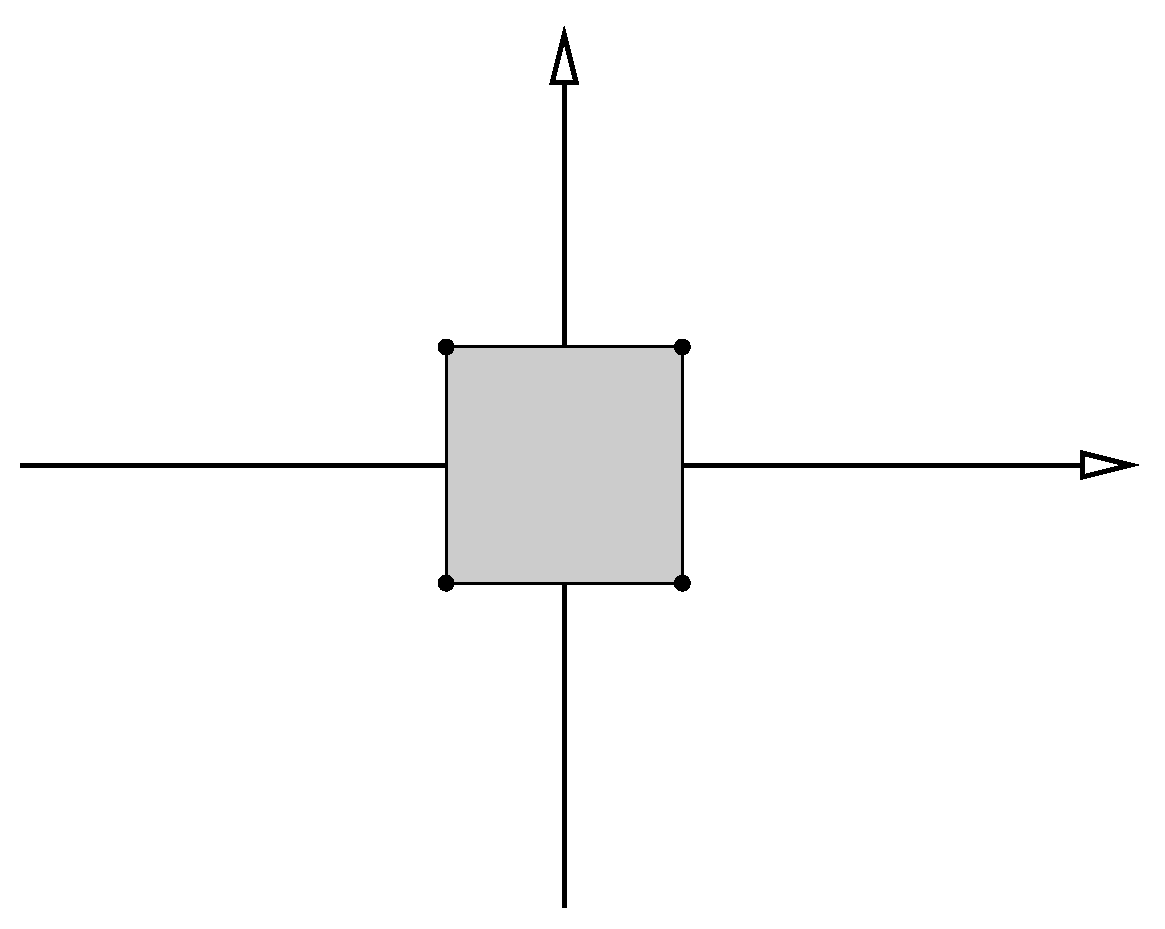
\includegraphics[width=10cm]{./deformation.eps}}
    \put(9.5,3.3){$x$}
    \put(4.3,7.5){$y$}
    \put(3.7,5.6){$A$}
    \put(5.8,5.6){$B$}
    \put(3.2,5.2){$(-1,1)$}
    \put(5.5,5.2){$(1,1)$}
    \put(3.6,2.4){$D$}
    \put(5.7,2.4){$C$}
    \put(2.9,2){$(-1,-1)$}
    \put(5.2,2){$(1,-1)$}
  \end{picture}
  \caption{\'El\'ement de volume \`a l'instant initial.}
  \label{fig:deformation}
\end{figure}
\item Comment pourrait-on g\'en\'erer ce type d'\'ecoulement ? Citer des
exemples d'\'ecoulements r\'eels pr\'esentant ces caract\'eristiques.
\end{enumerate}
}


%%%%%%%%%%%%%%%%%%%%%%%%%%%%%%%%%%%%%%%%%%%%%%%%%%%%%%%%%%%%%%%%%%%%%%
\subsection{Descriptions lagrangienne et eul\'erienne 
{\small \it (Partiel 2004)}}
%%%%%%%%%%%%%%%%%%%%%%%%%%%%%%%%%%%%%%%%%%%%%%%%%%%%%%%%%%%%%%%%%%%%%%


On consid\`ere l'\'ecoulement suivant donn\'e sous forme 
\textit{lagrangienne} :
\begin{equation*}
\left\{
\begin{array}{rcl}
X(t) & = & b t + X_0 \\
Y(t) & = & \frac{a}{\omega} \sin(\omega t) + Y_0
\end{array}
\right.
\text{o\`u $a$, $b$ et $\omega$ sont des constantes.}
\end{equation*}
\begin{enumerate}
\item Donner l'\'equation des trajectoires $Y(X)$.
\item Donner la signification physique de $X_0$ et $Y_0$.
\item Calculer l'acc\'el\'eration lagrangienne $\vec{a}_L$.
\item Donner la description eul\'erienne de ce mouvement.
Calculer le terme convectif. En d\'eduire l'acc\'el\'eration
eul\'erienne $\vec{a}_E$. Comparer avec $\vec{a}_L$.
\item Ce mouvement est-il stationnaire ? isovolume ? irrotationnel ?
\item D\'eterminer l'\'equation des lignes de courant. On en pr\'ecisera
la forme g\'eom\'etrique.
\item Tracer les trajectoires correspondant aux trois conditions initiales :
$X_0 = 0$ et $Y_0 = -1, 0$ et $1$.
\item Tracer sur le m\^eme graphe les lignes de courant pour $y_0 = -1, 0$
et $1$ aux instants $t = 0, 0.5$ et $1$ seconde. On prendra 
$b = 1$ m.s$^{-1}$, $a = 2 \pi$ m.s$^{-1}$ et $\omega = 2 \pi$ rad.s$^{-1}$.
\end{enumerate}



%%%%%%%%%%%%%%%%%%%%%%%%%%%%%%%%%%%%%%%%%%%%%%%%%%%%%%%%%%%%%%%%%%%%%%%%%%%
\subsection{\'Ecoulement instationnaire accéléré}
%%%%%%%%%%%%%%%%%%%%%%%%%%%%%%%%%%%%%%%%%%%%%%%%%%%%%%%%%%%%%%%%%%%%%%%%%%%


On consid\`ere l'\'ecoulement plan \textit{instationnaire} d\'efini
par $u = 1$ et $v = t$.
\begin{enumerate}
\item V\'erifier que l'\'ecoulement est incompressible.
\item D\'eterminer :
  \begin{itemize}
  \item[$\bullet$] les lignes de courant,
  \item[$\bullet$] les trajectoires,
  \item[$\bullet$] les lignes d'\'emission.
  \end{itemize}
\end{enumerate}




% !TEX root = TD_fluides_part1.tex


\section{Ecoulements visqueux I : Rhéologie et écoulements stationnaires parallèles}


\setcounter{subsection}{-1}

\subsection{Ecoulement de Poiseuille} 

{\em (exercice préparatoire, correction sur moodle)} 


%--------------------------------------------------------------------------------------------------
\subsection{Ecoulement de dentifrice}
%--------------------------------------------------------------------------------------------------

Le dentifrice est un exemple de "fluide \`a seuil" qui ne s'\'ecoule que si la contrainte 
de cisaillement est sup\'erieure \`a un seuil $\tau_c$. 
Consid\'erons donc un tube cylindrique de longueur $L$ rempli de dentifrice, et soumis \`a 
une diff\'erence de pression $p_e - p_s$. 
\begin{enumerate}
\item 
  D\'eterminer le profil de la contrainte de cisaillement dans le tube. 
\item 
  A partir de quelle diff\'erence de pression le dentifrice s'\'ecoule-t-il ? 
\item 
  Etablir l'expression du champ des vitesses, et repr\'esenter ce champ. 
\item 
  Etablir l'expression du d\'ebit en fonction du gradient de pression. 
\end{enumerate}



%--------------------------------------------------------------------------------------------------
\subsection{Film de peinture (Partiel 2018)}
%--------------------------------------------------------------------------------------------------

On consid\`ere un liquide de masse volumique $\rho$ uniforme qui s'écoule 
sous la forme d'un film d'\'epaisseur uniforme $h$ sur un plan inclin\'e 
d'un angle $\theta$ par rapport \`a l'horizontale. On introduit un repère $(x,y)$ où la direction 
$x$ est alignée avec le plan incliné et $y$ est la direction perpendiculaire.

%Soit $q$ le d\'ebit-volume impos\'e par unit\'e de largeur. 

Dans cet exercice on repartira de l'équation de Cauchy écrite sous la forme suivante :

$$
\rho \frac{ d \vec{u}}{d t}  =  \rho \vec{ g} - \vec{grad} p + \vec{div} ( \mytensor{\tau} )
$$

\begin{enumerate}
\item 
Sous des hypothèses que vous préciserez, montrez que l'équation de Cauchy peut
se ramener à l'équation suivante :
$$ 
 0 =  \rho g \sin \theta + \frac{\partial \tau_{xy} }{\partial y}
$$
%$$
%0 =  - \frac{\partial p}{\partial y} + \rho g \cos \theta 
%$$

\item 
Après avoir précisé la condition limite vérifiée par la contrainte en $y=h$,  établir la loi 
$\tau_{xy}(y)$ donnant la contrainte visqueuse dans le film. 

\item 
En déduire que la contrainte est maximale (en module) à la base du film et vaut :
$$ 
\tau_{xy}(y=0)  = - \rho g h \sin \theta 
$$ 
Donnez une interprétation simple de cette expression.

\item Dans le cas d'un fluide Newtonien, justifiez que la loi de vitesse $u(y)$ 
correspond à un polynôme d'ordre 2, et tracez la forme du profil $u(y)$ correspondant
(on ne demande pas la résolution mathématique complète du problème).

Dans la suite on considère le cas d'un fluide non Newtonien obéissant à la loi de Bingham:
$$
\frac{\partial u}{\partial y }  = 
\left\{ \begin{array}{ll}  0 & \quad (|\tau_{xy}| < \tau_c) \\  
\frac{1}{\mu} (\tau_{xy}-\tau_c) & \quad ( \tau_{xy} > \tau_c) \\
\frac{1}{\mu} (\tau_{xy}+\tau_c) & \quad ( \tau_{xy} < -\tau_c) 
\end{array}
\right.
$$ 

\item  Tracez la forme de la loi rhéologique ($\tau_{xy}$ en fonction de 
$\dot{\gamma} = \partial u/\partial y $) et comparez au cas d'un fluide Newtonien. Justifiez la désignation de "fluide à seuil" utilisée pour décrire ce type de fluide.

\item Montrez qu'il existe une épaisseur critique $h_c$ telle que si $h<h_c$ le film ne coule pas.
Exprimez $h_c$ en fonction de $\rho,g,\theta$ et $\tau_c$.

\item Dans le cas où $h>h_c$ tracez la forme attendue pour le profil de vitesse $u(y)$ 
(on ne demande pas une résolution mathématique complète du problème).

\item Application : 
On considère une peinture acrylique, décrite comme un fluide de Bingham avec les caractéristiques suivantes : $\tau_c = 1 Pa$ ; $\rho = 850 kg/m^3$; $\mu = 10^{-2} Pa \cdot s$. Donnez l'épaisseur maximale $h_c$ d'une couche de peinture sur une paroi verticale permettant d'éviter tout risque de coulure.

\end{enumerate}

% !TEX root = TD_fluides_part1.tex

\setcounter{section}{4}

\section{Ecoulements visqueux II : problèmes instationnaires}

\setcounter{subsection}{-1}

\subsection{Premier problème de Stokes} 

{\em (exercice préparatoire, correction sur moodle)} 



%\subsection{Second problème de Stokes}

%--------------------------------------------------------------------------------------------------
\subsection{Ecoulement au voisinage d'une paroi oscillante (second problème de Stokes)} \label{2pbStokes}
%--------------------------------------------------------------------------------------------------

On consid\`ere un fluide de viscosit\'e cin\'ematique $\nu$ occupant un demi-espace 
limit\'e par une plaque plane anim\'ee d'un mouvement oscillant sinuso\"{\i}dal $U \cos \omega t$, 
parall\`element \`a elle-m\^eme ("deuxi\`eme probl\`eme de Stokes"). 
%Montrer que le mouvement p\'en\^etre dans le fluide sur une distance $\delta = \sqrt{2\nu/\omega}$.
Retrouvez la loi $u(y,t)$ décrivant la structure de l'écoulement (cf. tableau "solutions exactes" en Annexe).

Déduisez-en la contrainte visqueuse exercée par le fluide sur la paroi, et montrez que celle-ci est donnée par la loi suivante :

\[
\color{black}{\tau_p  = - \frac{\mu U \sqrt{2}}{\delta} \cos (\omega t - \pi/4)}
\]

Que vaut la vorticité dans l'écoulement ? montrez que la vorticité à la paroi est directement reliée à la contrainte pariétale.




%--------------------------------------------------------------------------------------------------
\subsection{Rythmes cardiaques (TP numérique)}
%--------------------------------------------------------------------------------------------------

Outre une diff\'erence de pression moyenne,
le c{\oe}ur qui bat impose une variation p\'eriodique du gradient de
pression ce qui conduit \`a un \'ecoulement puls\'e dans les vaisseaux
sanguins.
L'objectif de cet exercice est de caract\'eriser ce type d'\'ecoulement
en particulier dans les limites des basses fr\'equences (organisme au repos) 
et hautes fr\'equences (activit\'e cardiaque intense).
 
Consid\'erons un \'ecoulement plan entre deux plaques planes distantes de $2h$
g\'en\'er\'e par un gradient de pression sinuso\"{\i}dal
\`a pulsation $\omega$ fix\'ee~:
\[
\dpa{p}{x} = K \cos\omega t.
\]

\begin{enumerate}
\item 
Dans l'hypoth\`ese d'un \'ecoulement plan parall\`ele, montrer que
la vitesse horizontale $u(y, t)$ v\'erifie l'\'equation
\begin{equation}
\underbrace{\rho \dpa{u}{t}}_{[I]} = \underbrace{- K \cos \omega t}_{[P]} + \underbrace{\mu \ddpa{u}{y}}_{[V]}
\label{eq:ns}
\end{equation}

\item Comparer l'ordre de grandeur des termes $[I]$ et $[V]$ dans l'équation précédente. Montrez que le rapport de ces deux termes fait apparaître 
le nombre de Stokes (ou nombre de Womersley) $St = \frac{\omega h^2  }{\nu}$.

\item Dans l'hypothèse $St \ll 1$, justifiez que l'écoulement correspond à chaque instant à l'écoulement de Poiseuille plan   
(régime quasi-statique).

\item Dans l'hypothèse $St \gg 1$, l'analyse des ordres de grandeur suggère qu'on peut dans une première approximation
négliger le terme visqueux. Quelle est alors la solution du problème ? celle-ci est-elle valide dans la totalité du domaine ?

\item Toujours dans le cas  $St \gg 1$, justifiez qu'il existe une {\em couche limite} dans laquelle le terme visqueux ne peut être négligé. 
Quelle est l'épaisseur de cette couche limite ?

\item $^*$ Dans le cas général ($St = {\mathcal O}(1)$, montrez que la solution du problème peut se mettre sous la forme suivante :
$$u(y, t) = Re \left \{  \underline{U}(y) \e^{\im \omega t} \right \}.$$

Avec 

\begin{equation}
\label{sol}
 \underline{U}(y) = \frac{iK}{\rho \omega} \left \{ 
1 - \frac{\cosh [ y ( 1+i) \sqrt{\omega / 2\nu} ]}{\cosh [ 
h ( 1+i) \sqrt{\omega / 2\nu} ]}
\right \}
\end{equation}

Indication : on utilisera la méthode de la variable complexe comme dans le cas de l'exercice précédent pour aboutir à une équation différentielle d'ordre 2 pour $ \underline{U}(y)$ que l'on résoudra en tenant compte des conditions aux limites du problème.

\item $^*$ Etudiez le comportement de l'expression précédente dans les limites  $\omega \rightarrow 0 $ et $\omega •\rightarrow \infty$, et montrez que l'on retrouve bien les prédictions obtenues précédemment dans les cas $St \ll 1$ et $St \gg 1$.

\end{enumerate}


%\begin{figure}[htb]
%  \begin{center}
 %   \begin{picture}(100, 30)(0, 50)
  %    \put(0, 0){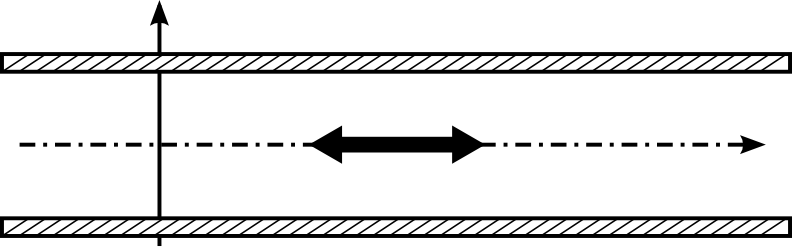
\includegraphics[width=10cm]{ecoulement_pulse_plan.png}}
  %    \put(14.5, 4.5){$-h$}
   %   \put(14.5, 18.5){$+h$}
   %   \put(35, 17){$\partial p/\partial x = K \cos \omega t$}
  %  \end{picture}
%  \end{center}
%  \mycaption{Ecoulement puls\'e en canal plan.}
%  \label{fig:ecoulement_pulse}
%\end{figure}


\Archives{
\subsection{Bulles de savons connectées par une paille}


\begin{center}
\input{Figures/Bibulle.pspdftex}
\end{center}
Deux bulles de savon sont connectées par un tube cylindrique de rayon $a$
et de longueur $L$. On note $R_1(t)$ et $R_2(t)$ les rayons (intérieurs)
respectifs des bulles, $e$ l'épaisseur du film de savon, $P_1$ et $P_2$ 
les pressions à l'intérieur de chacune des bulles, et $P_0$ la pression 
atmosphérique.
Les viscosités cinématique et dynamique de l'air sont notés 
respectivement $\nu$ et $\mu$, et la tension interfaciale 
de l'interface film de savon / air est notée $\gamma$.

On suppose que $R_1$ et $R_2$ sont grands devant $a$ ; ainsi
le volume d'air contenu dans la bulle 1 sera pris comme égal
au volume d'une sphère de rayon $R_1$ (de même pour la bulle 2).

On note $V_0$ le volume total d'air dans les bulles 1 et 2.





\begin{enumerate}

\item
Exprimez $P_1-P_0$ en fonction du rayon $R_1$ et de l'épaisseur
$e$ du film de savon. Simplifiez cette expression en supposant $e\ll R_1$.
Exprimez de même $P_2-P_0$ en fonction de $R_2$.
%\begin{enumerate}

\item Quelles sont les solutions d'équilibre du système ? La situation $R_1 = R_2$ est-elle une situation stable ?


%En reprenant
%le calcul précédent et en comparant l'ordre de grandeur des termes
%visqueux et instationnaire dans l'équation de Navier-Stokes,
%montrez que l'approximation quasi-statique utilisée précédemment
%est effectivement valide si $\tau \gg a^2/\nu$.


\item On note $[T]$ l'échelle de temps du problème (inconnue à ce stade de la modélisation). 
Sous quelle(s) hypothèse(s) peut-on négliger le terme instationnaire et le terme d'advection dans l'équation de Navier-Stokes ?
%est effectivement valide si $\tau \gg a^2/\nu$.
%\end{enumerate}


\item
Montrez que sous les hypothèses formulées à la question précédente, l'écoulement dans
le tube est donné à tout instant par la loi de Poiseuille, et que le débit volumique
dans le tube (compté algébriquement dans la direction allant de la bulle
1 à la bulle 2) est donné par la formule suivante :

$$
Q = \frac{\pi a^4}{8 \mu L} (P_1-P_2)
$$



\item Montrez que le rayon $R_1(t)$ obéit à l'équation 
différentielle suivante :

$$
- \frac{d}{dt} \left( \frac{4 \pi R_1(t)^3}{3} \right) 
= \frac{\pi a^4\gamma }{2 \mu L} \left[ \frac{1}{R_1(t)} -     \frac{1}{R_2(t)}  \right]
$$

\item Sous quelle(s) hypothèse(s) est-il justifié de supposer que le volume
total d'air dans les bulles 1 et 2 est conservé ?
%Exprimez dans ce cas $R_2$ en fonction de $R_1$ et $V_0$ (volume total).

\item Le système admet une position d'équilibre correspondant à $R_1 = R_2 = R_0$ 
et $V_0 = 8 \pi/3 R_0^3$. On suppose que le système s'écarte légèrement 
de cette position d'équilibre et qu'on a $R_1(t) = R_0 + r(t)$ et $R_2(t) = R_0 - r(t)$.

Montrez que sous l'hypothèse $r(t) \ll R_0$ cette situation traduit bien la conservation du volume total. 


\item Par un développement limité de l'équation précédente, montrez que $r(t)$ 
obéit à une équation différentielle de la forme suivante :

$$
\frac{dr}{dt} 
= \sigma r , \qquad  \mbox{ avec } \sigma = \frac{a^4 \gamma}{4 R_0^4 \mu L} 
$$

\item Donnez la solution de cette équation. Quelle échelle de temps $[T]$ caractérisant l'évolution du système cette solution met-elle en évidence ?

%Exprimez $\sigma$ en fonction des données du problème.
%Que peut-on en déduire sur la stabilité de la position d'équilibre ?

\item
On donne les valeurs suivantes : $a = 1mm$, $R_0 = 5cm$, $\nu = 10^{-6} m^2. s^{-1}$, 
$\rho = 1.26 kg. m^{-3}$, $\gamma = 0.07 N.m^{-1}$, $L=20cm$. Calculez l'échelle de temps $[T]$ d'évolution du système. 
L'hypothèse quasi-statique est-elle bien justifiée ?

\end{enumerate}
  }
 







% !TEX root = TD_fluides_part1.tex



\section{Ecoulements visqueux III : écoulements rampants}


\setcounter{subsection}{-1}

%--------------------------------------------------------------------------------------------------
\subsection{Amortisseur hydraulique (partiel 2017; correction sur moodle)}
%--------------------------------------------------------------------------------------------------

On consid\`ere un amortisseur constitu\'e d'un piston de rayon $R=20$ mm et de longueur $L=20$ mm coulissant dans un cylindre de rayon $R+a$, avec $a =0.1$ mm. Ce cylindre est rempli d'une huile de viscosit\'e dynamique $\mu=0.1$Pa.s.\\
On veut d\'eterminer la relation entre la force $F$ appliqu\'ee sur le piston et sa vitesse $V$ par rapport au cylindre. Le fluide dans les deux chambres sup\'erieure et inf\'erieure au piston sera consid\'er\'e au repos. L'\'ecoulement,dans l'interstice (le jeu) entre les parois lat\'erales du piston et du cylindre, est visqueux (newtonien), stationnaire et \'etabli . Il sera approxim\'e \textit{localement} par l'\'ecoulement \'etabli entre deux plaques planes distantes de $a$, de longueur $L$, de largeur $2\pi R$ (p\'erim\`etre {\it d\'eroul\'e}). On consid\'erera que les pressions $p_i$ et $p_a$ dans les chambres inf\'erieure et sup\'erieure sont uniformes, et que la contribution hydrostatique, d'ordre $\rho gL$, est n\'egligeable devant $p_i-p_a$.\\


\begin{figure}[hbt]
  \begin{center}
    \setlength{\unitlength}{1mm}
    \begin{picture}(100, 60)(0, 0)
      \put(0, 0){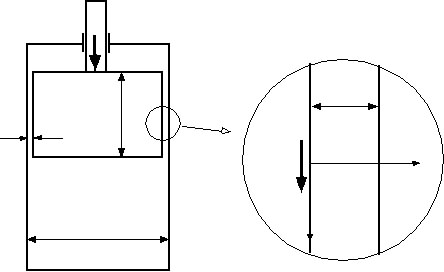
\includegraphics[width=10cm]{Figures/Amortisseur.jpg}}
      \put(1, 32){$a$}
      \put(20, 55){$F$}
      \put(23, 34){$L$}
      \put(15, 9){$2(R+a)$}
      \put(10, 48){$p_a$}
      \put(20, 20){$p_i$}
      \put(66, 10){$x$}
      \put(89, 27){$y$}
      \put(63, 25){$V$}
      \put(76, 39){$a$}
    \end{picture}
  \end{center}
  \label{fig:amortisseur}
  \caption{Sch\'ema de l'amortisseur hydraulique.}
\end{figure}

\begin{enumerate}
\item 
  On cherche une solution « plane » $u=u(y)$  avec $y=r-R$ pour la vitesse axiale dans l’interstice entre le piston et le cylindre.  Expliquer succinctement pourquoi on peut négliger localement les effets de courbure sur le profil de vitesse et approximer $u$ par $u(y)$ (au lieu de $u(r,\theta,x)$ !)

%\rep{}
  
\item 
Montrer que dans le jeu (interstice) entre le piston et le cylindre l'écoulement est gouverné par le système différentiel  
$$
-\frac{\partial p}{\partial x} + \mu \frac{\partial^2 u}{\partial y^2} = 0 ;\quad \frac{\partial p}{\partial y}=0
$$

\rep{Ayant justifié que le profil est de la forme $\myvec{u} = [u(y), 0, 0]$ , on injecte cette solution dans les équations de Navier-Stokes.  En ne gardant que les termes non nuls, on aboutit aux équations demandées.}


 Qu'en déduit-on sur la pression et son gradient suivant $x$ ?

\rep{ En dérivant la première équation selon $x$ on a  $\frac{\partial^2 p}{\partial x^2}=0$. La pression est une fonction linéaire de $x$ et son gradient est constant.
} 

\item 
Établir l'expression du profil de vitesse $u(y)$ et montrer qu'il correspond à la somme d'un écoulement de Poiseuille proportionnel à $-\partial p/\partial x$ et d'un écoulement de Couette proportionnel à $V$. 

\rep{
En intégrant deux fois selon $y$ et en tenant compte des conditions limites $u(0)= V$ et $u(a) = 0$, on trouve : 
$$ 
u(y) = V \cdot \left( 1 - \frac{y}{a} \right) + \frac{a^2}{2\mu} \frac{\partial p}{\partial x} \frac{y}{a} \left( 1 - \frac{y}{a} \right)   
$$
On reconnait un écoulement de Couette et un écoulement de Poiseuille.
}


\item Calculez le débit volumique à travers l'interstice. On distinguera la contribution $Q_p$  associée à l'écoulement de Poiseuille et la contribution $Q_c$ associée à l'écoulement de Couette.

\rep{
Ce débit (compté du bas vers le haut) vaut :
$$
Q = - \int_R^{R+a} u(r) 2 \pi r dr d \theta \approx - L \int_0^a u(y) dy = Q_c + Q_p
$$ 
$$ 
\mbox{ avec } Q_c = -\frac{V L a}{2} ; \quad Q_p = -\frac{a^2 L}{12 \mu}  \frac{\partial p}{\partial x}
$$
}

%\i

\item Montrer que le débit volumique chassé par le piston est égal à $Q = \pi R^2 V$.

\rep{Au cours d'un instant $dt$ le piston chasse un volume $d{\cal V} = \pi R^2 V dt$ vers le haut, 
le débit volumique est donc $Q = d{\cal V}/dt = \pi R^2 V$.}


\item En déduire que le gradient de pression est donné (à l'ordre dominant) par 
$(p_i-p_a)/L = 6 \mu R V/a^3$ .

On justifiera au passage que le débit associé à l'écoulement de Couette est négligeable devant celui associé à l'écoulement de Poiseuille.

\rep{ 
On écrit maintenant $Q = Q_p+ Q_v$, ce qui conduit à :
$$
\frac{\partial p}{\partial x} = \frac{6\mu R V}{a^3} \left( 1+\frac{a}{R} \right)  \approx  \frac{6\mu R V}{a^3}
$$
Le terme négligé $a/R$ correspond effectivement au rapport $Q_c/Q$.
}





\item  Montrez que la force exercée sur le piston se compose de trois termes, notés respectivement $F_P$ (résultante des efforts de pression), $F_{v,c}$ (résultante des contraintes visqueuses associées à l'écoulement de Couette), et $F_{v,p}$ (résultante des contraintes visqueuses associées à l'écoulement de Poiseuille).

Exprimez $F_p, F_{v,c}$ et $F_{v,p}$ en fonction des données du problème.

\rep{
$$
\myvec{F} = \int_S (-p \myvec{n} + \tau \cdot \myvec{n} ) dS   
$$
En projetant selon l'axe $x$ on a $F = F_p+F_{v,c}+F_{v,p}$ avec respectivement :
$$
F_p = 6 \pi \mu V \frac{R^3}{a^3} ; \quad 
F_{v,p} = 12 \pi \mu L V R^2/a^2 ; \quad 
F_{v,c} = 2 \pi \mu L V R/a.
$$
}

\item Comparez l'ordre de grandeur de ces trois forces, et montrez qu'à l'ordre dominant la force totale a pour expression $F = 6 \pi \mu V \frac{R^3}{a^3}$.

\rep{C'est la contribution $F_p$ qui domine.}

\item Application : Quelle force faut-il appliquer pour imprimer une vitesse de $1cm/s$ au piston ? L’écoulement est-il laminaire ? 

\rep{ $F =1.5\cdot 10^5 N$, force équivalant à 15 tonnes ! 
Le Reynolds est de l'ordre de la centaine, l'écoulement reste donc laminaire.}


%\item  Calculer les contraintes de cisaillement liées d’une part à l’écoulement de couette et d’autre part à l’écoulement de Poiseuille. Sont-elles du même ordre ? Laquelle a été négligée dans le calcul de la force F appliquée au piston ?

\end{enumerate}



%--------------------------------------------------------------------------------------------------
\subsection{Drainage entre deux disques rapproch\'es (d'apr\`es examen 2004) \exonormal}
%--------------------------------------------------------------------------------------------------

Deux disques circulaires plans de rayon $R=5$ cm sont dispos\'es parall\`element 
(fig.~\ref{fig:disques}) l'un au-dessus de l'autre. 
Dans l'espace entre les disques se trouve une huile de viscosit\'e dynamique $\mu = 6.26$ Pa s 
et de masse volumique $\rho = 1230$ kg/m$^3$. 
On consid\`ere que l'\'epaisseur de fluide $h$ entre les deux disques reste tr\`es petite 
devant le rayon $R$ : $h \ll R$. L'\'epaisseur $h_0$ \`a l'instant initial ($t=0$) est \'egale 
\`a $h_0=0,5$ cm. La pression \`a l'ext\'erieur des disques correspond \`a la pression 
atmosph\'erique $P_a$.

On exerce une force $\textbf{F} = F \textbf{e}_z$ sur le disque sup\'erieur afin de 
chasser lat\'eralement le fluide. Cette force impose au disque sup\'erieur une vitesse 
$\textbf{U} = U \textbf{e}_z$, le disque inf\'erieur restant fixe.

Dans un premier temps, on se propose de d\'eterminer l'intensit\'e $F(t)$ de la force qu'il faut 
exercer pour maintenir \emph{constante} la vitesse $U = 0,5$ mm/s du disque sup\'erieur. 
On s'attachera ensuite \`a d\'ecrire en d\'etail l'\'ecoulement entre les deux disques.

La couche de fluide \'etant mince et le probl\`eme axisym\'etrique, on consid\`ere que 
la pression ne d\'epend ni de $z$ ni de l'angle azimutal $\theta$, soit $p = p(r, t)$, 
et on cherche un champ de vitesse s'\'ecrivant : 
$\textbf{u} = u_r(r, z, t) \textbf{e}_r + u_z(r, z, t) \textbf{e}_z$.

\begin{figure}[hbt]
    \setlength{\unitlength}{1mm}
  \begin{center}
    \begin{tabular}{cc}
      \begin{picture}(75, 60)
	\put(0, 0){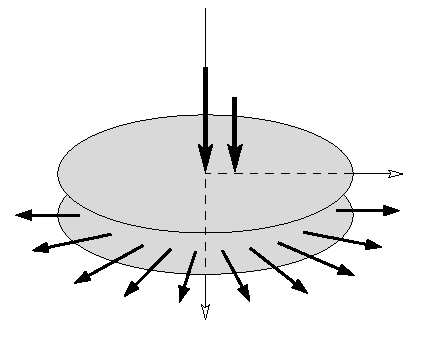
\includegraphics{disques1}}
	\put(60, 40){$P_a$}
	\put(31, 3){$z$}
	\put(65, 32){$r$}
	\put(30, 45){$\textbf{F}$}
	\put(42, 40){$\textbf{U}$}
      \end{picture}
      &
      \begin{picture}(75, 60)
	\put(0, 0){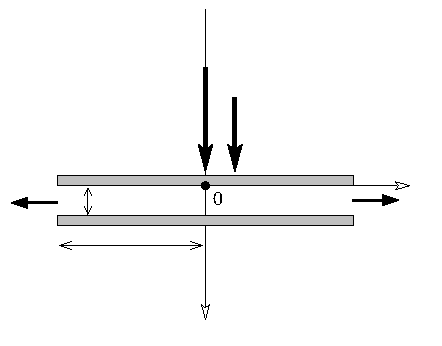
\includegraphics{disques2}}
	\put(20, 13){$R$}
	\put(65, 30){$r$}
	\put(30, 5){$z$}
	\put(17, 23.5){$h(t)$}
	\put(10, 35){$P_a$}
	\put(30, 45){$\textbf{F}$}
	\put(42, 40){$\textbf{U}$}
      \end{picture}
    \end{tabular}
  \end{center}
  \mycaption{Ecoulement visqueux entre deux disques.}
  \label{fig:disques}
\end{figure}

Les relations ci-dessous donnent, en coordonn\'ees cylindriques
$(r, \theta, z)$, la composante radiale de l'\'equation du mouvement
(\ref{eq:mvt}) et l'\'equation d'incompressibilit\'e (\ref{eq:cont}) : 
\begin{eqnarray}
\rho \left [  \dpa{u_r}{t} + u_r \dpa{u_r}{r} + u_z \dpa{u_r}{z} \right ]
&=& - \dpa{p}{r} + \mu \left[ 
\dpa{}{r} \left( \frac{1}{r}\dpa{}{r}(r u_r) \right) + \ddpa{u_r}{z} \right],
\label{eq:mvt} \\
\frac{1}{r} \dpa{}{r}(r u_r) + \dpa{u_z}{z} & = & 0.
\label{eq:cont}
\end{eqnarray} 

\begin{enumerate}
\item
  \begin{enumerate}
  \item 
    En choisissant $U$, $R$  et $[T] = R/U$ respectivement comme \'echelles caract\'eristiques
    de vitesse, de longueur et de temps, calculer la valeur du nombre de Reynolds et du nombre de Stokes pour cet \'ecoulement. Commenter.
  \item 
    Montrer que l'\'equation du mouvement peut se simplifier sous la forme :
    \begin{equation}
      \dpa{p}{r} = \mu \left[ \dpa{}{r} \left( \frac{1}{r}\dpa{}{r}(r u_r) \right) +
	\ddpa{u_r}{z} \right].
      \label{eq:smpl}
    \end{equation}
  \item 
    On cherche \`a simplifier davantage l'\'equation ci-dessus.
    En choisissant comme \'echelles de longueur $h$ suivant $z$, et $R$
    suivant $r$, pour estimer l'ordre de grandeur des d\'eriv\'ees partielles, 
    et sur la base de l'hypoth\`ese simplificatrice $h \ll R$, simplifier le terme de droite 
    de l'\'equation (\ref{eq:smpl}). A l'aide des conditions aux limites (adh\'erence aux parois), 
    en d\'eduire l'expression de la vitesse radiale $u_r$ en fonction du gradient radial 
    de pression:      
  \begin{equation}
    u_r(r, z, t) = \frac{1}{2\mu} z [z-h(t)] \dpa{p}{r}.
  \end{equation}
      \end{enumerate}
\item 
  \begin{enumerate}
  \item 
    En injectant cette expression dans l'\'equation d'incompressibilit\'e
    (\ref{eq:cont}), d\'eterminer $u_z(r, z, t)$ en fonction de $\mu$, $h$,
    $\partial p/\partial r$ et $\partial^2 p/\partial r^2$.
  \item 
    A l'aide des conditions aux limites sur $u_z$ en $z=0$ et $z = h(t)$, 
    en d\'eduire l'\'equation diff\'erentielle que doit v\'erifier $p$.
  \item 
    Montrer alors que la pression au sein du fluide a pour expression :
    \begin{equation}
      p(r, t) = P_a + \frac{3\mu U}{h(t)^3} (R^2 - r^2).
      \label{pression}
    \end{equation}
  \end{enumerate}
\item
  \begin{enumerate}
  \item 
    D\'eterminer le module $F$ de la force pressante n\'ecessaire pour maintenir
    la vitesse $U$.
  \item 
    Donner l'expression de $h(t)$ en fonction de $U$ et $h_0$.
  \item 
    Tracer et commenter la courbe $F(t)$.
  \item 
    Sachant que le disque sup\'erieur sch\'ematise le piston d'un v\'erin qui admet
    pour pression maximale $P_m = 10^7$ Pa, d\'eterminer l'\'epaisseur minimale
    $h_m$ de fluide que l'on ne peut \'eliminer en maintenant la vitesse $U$, et le temps 
    $t_m$ n\'ecessaire pour effectuer cette vidange partielle de l'interdisque. 
    Faire l'application num\'erique.
  \end{enumerate}
\item
  \begin{enumerate}
  \item 
    Connaissant dor\'enavant le champ de pression (\ref{pression}) dans l'\'ecoulement, 
    d\'eterminer compl\`etement la vitesse radiale $u_r$ en tout point
    ($r$, $z$) de l'interdisque.
  \item
    Tracer la courbe donnant le profil de vitesse $u_r$ en fonction de la variable
    sans dimension $z/h$ pour diff\'erentes valeurs du temps $t$
    ($0 \leq t \leq t_m$).
  \item
    Etablir l'expression de la composante axiale de la vitesse, $u_z(r, z, t)$.
  \item
    D\'eterminer la tangente de l'angle ($\beta$) que fait le vecteur vitesse
    du fluide avec le plan  horizontal.
    En d\'eduire sch\'ematiquement l'allure des lignes de courant dans
    l'interdisque.
  \end{enumerate}
\item
  \begin{enumerate}
  \item 
    D\'eterminer le d\'ebit volumique de fluide s'\'ecoulant \textit{radialement}
    vers l'ext\'erieur des deux disques. Discuter le r\'esultat obtenu.
  \item 
    D\'eterminer le d\'ebit volumique de fluide s'\'ecoulant \`a travers une
    section normale \`a l'axe des disques (autrement dit, \textit{horizontale}).
    Tracer ce d\'ebit en fonction de $z/h$ et commenter.
  \end{enumerate}
\end{enumerate}



%--------------------------------------------------------------------------------------------------
\subsection{Coulée de lave}
%--------------------------------------------------------------------------------------------------

\noindent
On considère une coulée de lave le long d'une pente d'angle $\alpha$ par rapport à l'horizontale
(fig.~\ref{fig:Huppert}a).
Cet écoulement de lave est de faible épaisseur par rapport à sa longueur, et prend la forme d'un film mince
dont la surface libre est donnée par $y=h(x, t)$, où $y$ est la direction perpendiculaire à la pente de direction $x$.
Sous l'effet de la pesanteur, la coulée s'étale en s'écoulant, entre les points d'abscisses $x=0$ et $x=X(t)$,
ce dernier correspondant au front de la coulée.
L'objectif est ici de déterminer la loi de propagation du front de la coulée.

\begin{figure}[htb]
  \begin{center}
    \setlength{\unitlength}{1mm}
    \begin{picture}(160, 35)(0, -2)
      \put(0, 0){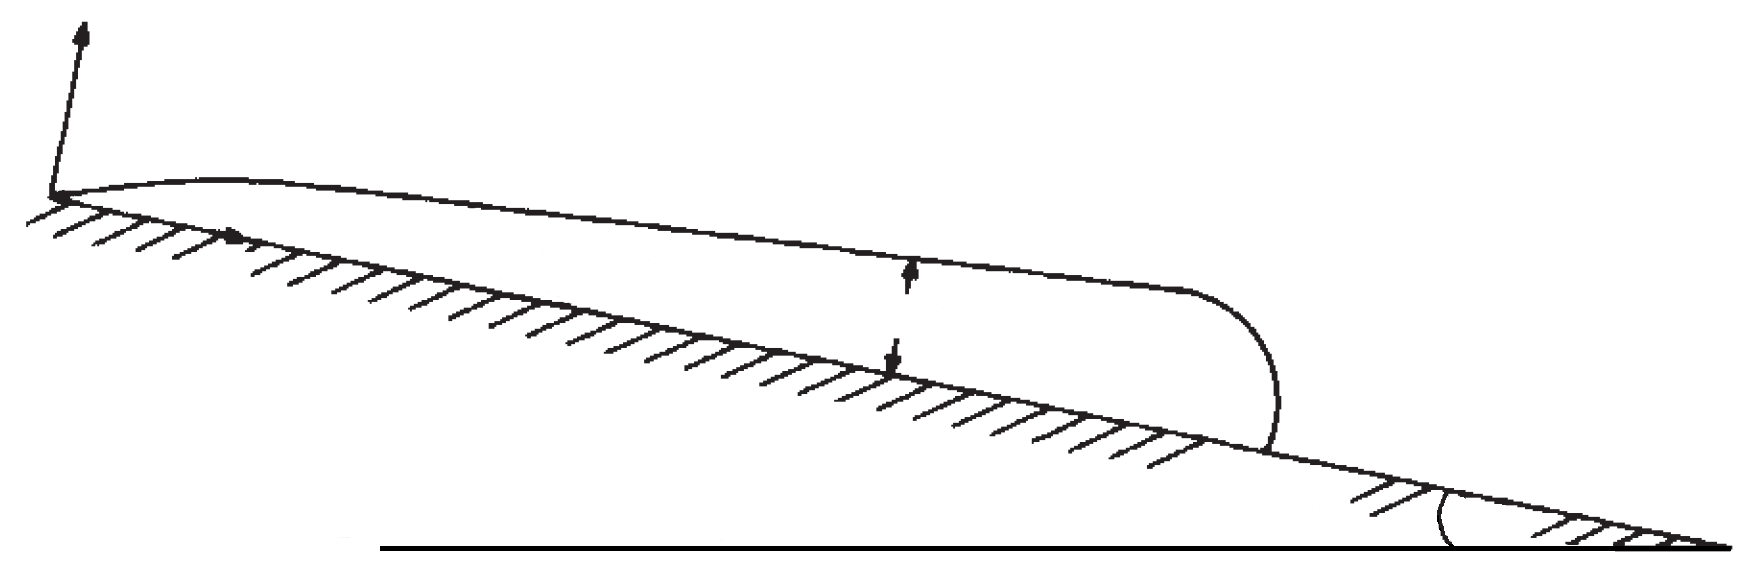
\includegraphics[width=9cm]{Huppert_geometry_clean.png}}
      \put(45, -6){(a)}
      \put(10.5, 15){\footnotesize $x$}
      \put(1, 27){\footnotesize	$y$}
      \put(0.5, 19){\footnotesize	$0$}
      \put(41.5, 13){\footnotesize $h(x, t)$}
      \put(60, 3.5){\footnotesize $X(t)$}
      \put(74.5, 2.4){\footnotesize $\alpha$}
      \put(70, 25){\thicklines \vector(0, -1){10}}
      \put(20, 22){\footnotesize $P_a$}
      \put(72, 20){\footnotesize $\myvec{g}=-g\,\myvec{e}_z$}
      \put(95, 1){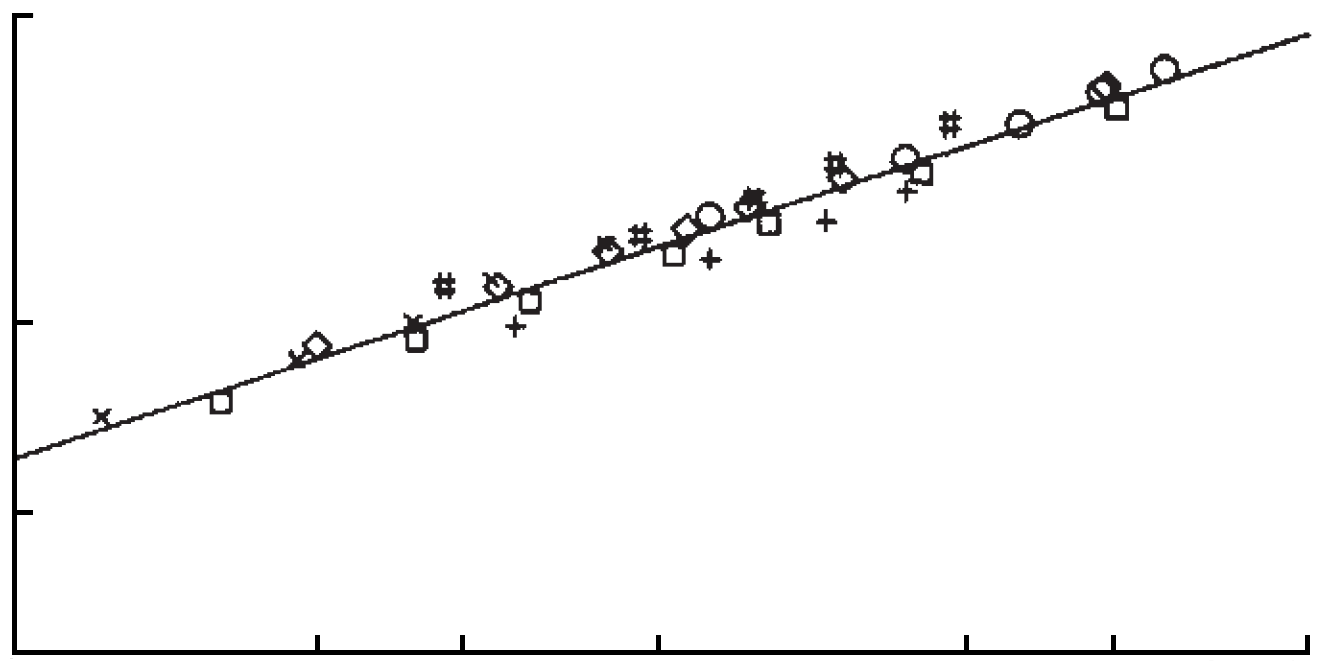
\includegraphics[width=6.5cm]{Huppert_results_clean.png}}
      \put(125, -6){(b)}
			\put(97, 30){\scriptsize $X(t)/\sqrt{S}$}
			\put(140, 4){\scriptsize $(g\sqrt{S}\sin\alpha/\nu)\, t$}
			\put(93, 0.7){\scriptsize $3$}
			\put(93, 7.7){\scriptsize $5$}
			\put(91.5, 16.9){\scriptsize $10$}
			\put(91.5, 31.9){\scriptsize $30$}
			\put(94, -2){\scriptsize $10^2$}
			\put(107, -2){\scriptsize $3.10^2$}
			\put(115, -2){\scriptsize $5.10^2$}
			\put(125, -2){\scriptsize $10^3$}
			\put(139, -2){\scriptsize $3.10^3$}
			\put(147, -2){\scriptsize $5.10^3$}
			\put(157, -2){\scriptsize $10^4$}
    \end{picture}
  \end{center}
  \mycaption{(a) : schéma de la coulée de lave. (b) : comparaison entre expérience (symboles) et prédiction théorique 
  	(droite de pente $1/3$ en échelle logarithmique). D'après Huppert (\textit{Nature} \textbf{300}, 427--429, 1982). }
  \label{fig:Huppert}
\end{figure}

\noindent
On supposera en première approximation que la lave est constituée d'un fluide homogène, 
de masse volumique $\rho$ uniforme, et newtonien, de viscosité cinématique $\nu$.
Dans l'hypothèse d'un écoulement incompressible, il est possible d'utiliser dans cette
configuration les équations de film mince pour la vitesse 
$\myvec{u} = u(x, y, t) \, \myvec{e}_x + v(x, y, t) \, \myvec{e}_y$
et la pression motrice $\hat{p} = p - \rho \, \myvec{g}\cdot \myvec{x}$ au point $\myvec{x}$ de coordonnées $(x, y)$~:
\[
	(1)\quad \frac{\partial^2 u}{\partial y^2} = \frac{1}{\mu} \, \frac{\partial \hat{p}}{\partial x},
	\qquad 
	(2)\quad \frac{\partial \hat{p}}{\partial y} = 0,
	\qquad
	(3)\quad \frac{\partial u}{\partial x} + \frac{\partial v}{\partial y} = 0,
	\quad \mbox{où $\mu = \rho \nu$ désigne la viscosité dynamique.}
\]
\begin{enumerate}
\item
	Montrer que la pression motrice s'écrit $\hat{p} = p(x, y, t) + \rho g (y\cos\alpha - x\sin\alpha)$.
\item
	En écrivant la continuité de la pression à l'interface $y=h(x, t)$, déduire de l'équation (2) 	
	que la pression au sein de la coulée a pour expression $p(x, y, t) = P_a + \rho g \cos\alpha\left [h(x, t)-y\right ]$ 
	où $P_a$ désigne la pression atmosphérique.
	En déduire la pression motrice $\hat{p}$.
\item
	Dans l'hypothèse de film mince, on peut supposer que $|\partial h/\partial x| \ll \tan\alpha$ pour $\alpha>0$.
	Montrer alors que $\partial \hat{p} / \partial x = -\rho g \sin\alpha$ en première approximation.
\item
	Dans ces conditions, résoudre l'équation (1) et montrer que $u(x, y, t) = -g\sin\alpha\; y^2/2\nu + A y + B$ où $A$ et $B$ sont
	deux fonctions de $x$ et $t$ à déterminer d'après les conditions aux limites en $y=0$ et $y=h(x, t)$.
	On négligera les frottements de l'air sur la coulée de lave.
\item
	Calculer le débit volumique le long de la coulée de lave : $q(x, t) = \displaystyle \int_0^{h(x, t)} u(x, y, t)\, dy$.
\item
	Montrer que la conservation de la masse implique que $\displaystyle \frac{\partial h}{\partial t} = -\frac{\partial q}{\partial x}$.
	On pourra admettre ce résultat.
\item
	Déduire des questions précédentes que $h(x, t)$ vérifie l'équation : 
	$\displaystyle \frac{\partial h}{\partial t} + \frac{g\sin\alpha}{\nu} h^2 \frac{\partial h}{\partial x} =0$.
\item
	Aux temps longs, on peut rechercher une solution, dite \textit{autosimilaire}, de la forme $h(x, t) = h_0\sqrt{x/t}$
	où $h_0$ est à déterminer en injectant ce type de solution dans l'équation pour $h$.
\item
		Le volume de cette coulée de lave étant fixé, $\displaystyle S = \int_0^{X(t)} h(x, t) \, dx$ est une constante du problème.
\item[]
		En déduire que la loi de propagation du front de lave s'écrit $X(t) = \sqrt{S} \; (t/\tau)^{1/3}$ 
		où $\tau$ est un temps caractéristique à déterminer en fonction des paramètres du problème (cf. fig.~\ref{fig:Huppert}b).	
\end{enumerate}

\hfill \textsl{(d'apr\`es partiel 2011)}

\Archives{
%--------------------------------------------------------------------------------------------------
\subsection{Ecoulement d'un film liquide d'\'epaisseur uniforme \exonormal}
%--------------------------------------------------------------------------------------------------

On consid\`ere un film liquide d'\'epaisseur uniforme s'\'ecoulant sur un plan inclin\'e 
d'un angle $\theta$ par rapport \`a l'horizontale. 
Soit $q$ le d\'ebit-volume impos\'e par unit\'e de largeur. 

\begin{enumerate}
\item 
  D\'eterminer le profil des vitesses $u(y)$ en fonction de l'\'epaisseur $h$.
\item 
  D\'eterminer l'\'epaisseur $h$ du film en fonction du d\'ebit $q$, 
  ainsi que la vitesse maximale $u_{max}$ et la vitesse moyenne $U$.
\item[]
  On définit le nombre de Reynolds du film par $Re = \rho u_{max}h/\mu$
  et une analyse de stabilit\'e linéaire du film uniforme montre que l'écoulement est stable 
  si $$Re < Re_c = \dfrac{5}{4\tan \theta}$$
  (au-del\`a une petite perturbation est amplifi\'ee et des vagues apparaissent).
\item
  Quel est le d\'ebit maximal d'un film stable sur un plan inclin\'e de 30 degr\'es ? 
  Un film vertical peut-il \^etre stable ?
\item 
  Une qualit\'e essentielle d'une bonne peinture est qu'une fois appliqu\'ee sur son support, 
  elle ``ne coule pas''. 
  Ceci peut \^etre r\'ealis\'e si la peinture n'est pas un fluide newtonien, 
  et ne s'\'ecoule que si la contrainte de cisaillement est sup\'erieure \`a un seuil. 
  Si le seuil d'\'ecoulement est $\tau_c = 1$ Pa, 
  quelle est l'\'epaisseur maximale d'une couche de peinture ne coulant pas sur un mur vertical ?
\end{enumerate}
}


%--------------------------------------------------------------------------------------------------
\subsection{Drainage d'un film liquide sur une paroi verticale \exonormal}
%--------------------------------------------------------------------------------------------------

Un plan rigide mouill\'e par un mince film liquide d'\'epaisseur uniforme 
est dress\'e verticalement; le liquide est alors drain\'e vers le bas par la gravit\'e. 

\begin{enumerate}
\item 
  Montrer que l'\'epaisseur $h$ \`a la distance $x$ du bord sup\'erieur de la plaque 
  satisfait l'\'equation approch\'ee % Batchelor p. 263
  $$
  \dpa{h}{t} + V \frac{h^2}{h_0^2} \dpa{h}{x} = 0,
  $$
  o\`u $V = \rho g h_0^2 / \mu$.
\item 
  Montrer qu'\`a l'instant t apr\`es le d\'ebut du drainage
  $$
  h = h_0 \sqrt{x/Vt} \quad \textrm{pour} \quad x \le Vt, 
  \qquad h = h_0 \quad \textrm{pour} \quad x \ge Vt.
  $$
\end{enumerate}

\appendix

% !TEX root = TD_fluides_part1.tex


\appendix
\section{Exercices de synthèses et annales d'examens}





\subsection{Vitesse de gouttes et particules en chute libre (partiel 2017)}

%\section{Vitesse de gouttes et particules en chute libre}

On considère une particule sphérique $ {\cal S}$ de rayon $a$, volume $V = 4 \pi a^3/3$
et masse volumique $\rho_p$ qui se déplace verticalement sous l'effet de la gravité $g$ dans un fluide ${\cal F}$ de viscosité dynamique $\mu$ et masse volumique $\rho_f$ supposée uniforme.  

On cherche à estimer la vitesse finale $U$ de celle-ci ainsi que le temps caractéristique 
$[T] =  \tau$ au bout duquel cette vitesse est atteinte en supposant qu'elle est lâchée à vitesse initiale nulle à l'instant $t=0$.

\begin{enumerate}

\item Ecrire les équations de Navier-Stokes sous une forme faisant
intervenir la pression motrice $\hat{p} = p + \rho_f g z$. Quelle est l'interprétation ce cette quantité ?

\item Donnez l'expression générale, sous forme d'une intégrale, de la force exercée par le fluide sur la surface de la sphère, puis montrez que celle-ci peut se décomposer sous la forme suivante :
$$
\vec F_{{\cal F} -> {\cal S}} = \vec F_A + \vec F_h  \mbox{ avec } 
\vec F_A = - \rho_f g V \vec e_z  
\mbox{ et } 
\vec F_h
= \int_{\cal S} \left( -\hat{p} \vec n + \mytensor{\tau } \cdot \vec n \right) dS
$$
Quelle est l'interprétation respective des deux termes $\vec F_A$ et $ \vec F_h$ ?

%\begin{enumerate}
%\itùem
%\end{itemize}

\item
Donnez l'ordre de grandeur des 4 différents termes de l'équation de Navier-Stokes écrite à la question 1. 
(On notera $[\hat p]$ l'ordre de grandeur des variations de pression motrice au sein du fluide).


\item En comparant l'ordre de grandeur du terme visqueux et du terme convectif, donnez la condition, faisant intervenir un nombre sans dimension classique, pour laquelle ce second 
terme peut être négligé.

On supposera dans la suite cette condition satisfaite.

\item A l'aide du principe de moindre dégénérescence, donnez l'ordre de grandeur de la jauge de pression $[\hat p]$ et de l'échelle de temps $[T]$. Quelle échelle de temps caractéristique reconnait-on dans cette dernière expression ?

\item Justifiez que l'ordre de grandeur du terme $\vec F_h$ vaut :
$$
[F_h]  \approx \mu a  U
$$
Que peut-on dire des contributions respectives de la pression motrice et de la contrainte visqueuse?
%exercée sur une particule sphérique est $F_z = 6 \pi \mu a  U$.



\item  
%Par un raisonnement dimensionnel, justifiez la forme de cette expression (on ne demande pas de démontrer le facteur $6\pi$). 
La résolution exacte des équations de Stokes autour d'une sphère permet de montrer le résultat suivant, que l'on admettra dans la suite :

$$|\vec F_h| = 6 \pi \mu a  U.$$


%\item
 Par un bilan des forces exercées sur la particule (son poids et la force exercée par le fluide exprimée selon la décomposition de la question 2), déterminez la vitesse de la particule prédite par cette formule dans les 4 cas suivants :

$(a)$ Gouttelette de brouillard ($a = 10 \mu m$, $\rho_p = 1000kg/m^3$) en chute dans de l'air ($\rho_f = 1.225 kg/m^3, \nu = 1.5\cdot 10^{-5} m^2/s$).

% Réponse : $U = 1.2 cm/s$ ; $Re = 7 \cdot 10^{-3}$.

%$(b)$ Bulle d'air ($a = 0.1mm$, $\rho_p = 1,225kg/m^3$) dans de l'eau douce ($\rho_p = 1kg/\ell$, $\nu= 10^{-6} m^2/s$).

% Réponse : $U = 2.02 cm/s$ ; $Re = 2$.


$(b)$ bille d'acier ($a= 1cm$, $\rho = 8.15 g/cm^3$) dans du miel ($\rho = 1.42 g/cm^3, \mu = 10 Pa \cdot s$) 

% Réponse : $U = 14.5 cm/s$ , $Re = 0.2$

%$(d)$ ballon de foot de rayon $a= 11cm$ et masse $m=425g$ en chute dans de l'air ($\rho_f = 1.225 kg/m^3$,  $\nu = 1.5\cdot 10^{-5} m^2/s$).

% Réponse : $U = 3558 m/s$, $Re = 26 \cdot 10^6$.

\item Calculez le nombre de Reynolds dans les cas $(a)$, $(b)$, $(c)$ et $(d)$. L'hypothèse faite à la question 4 est-elle justifiée ? Dans le cas contraire pensez-vous que la vitesse réelle est plus ou moins élevée que le calcul précédent ?

%\item Estimez le temps caractéristique $[T]$ 

%\item Dans le régime inertiel ($Re>1000$),  la formule de Stokes donnée à la question 2 peut être remplaçée par une loi empirique de la forme : $F_x = \frac{C_x}{2} \rho \pi a^2 U^2 $. 

%où $C_x$ est un coefficient (sans dimensions) qui vaut approximativement $0.5$.

%Justifiez par un raisonnement dimensionnel la forme de cette expression (on ne demande pas le calcul exact du $C_x$ !)

%\item Cette formule permet-elle de prédire une valeur plus réaliste de la vitesse pour un (ou plusieurs) des cas ($a-d$) discutés précédemment ?

%\item Dans les cas $(a)$ et $(b)$ Justifiez que la gouttelette et la bulle gardent  bien une forme sphérique au cours de leur mouvement.

%On donne la valeur de la tension de surface : $\gamma = 0.07 N/m$.

\end{enumerate}



	
	
	
	
			





%--------------------------------------------------------------------------------------------------
\subsection{Ecoulement autour d'un cylindre en rotation (d'après partiel 2010) \exonormal}
%--------------------------------------------------------------------------------------------------

On consid\`ere un cylindre solide de rayon $R$ et de grande longueur $L$
suivant son axe $Oz$, vertical.
Ce cylindre baigne dans un liquide de masse volumique $\rho$ et
de viscosit\'es cin\'ematique $\nu$ et dynamique $\mu$.

\begin{figure}[htb]
\begin{center}
\setlength{\unitlength}{1mm}
\begin{picture}(70, 50)(0, 0)
\put(0, 0){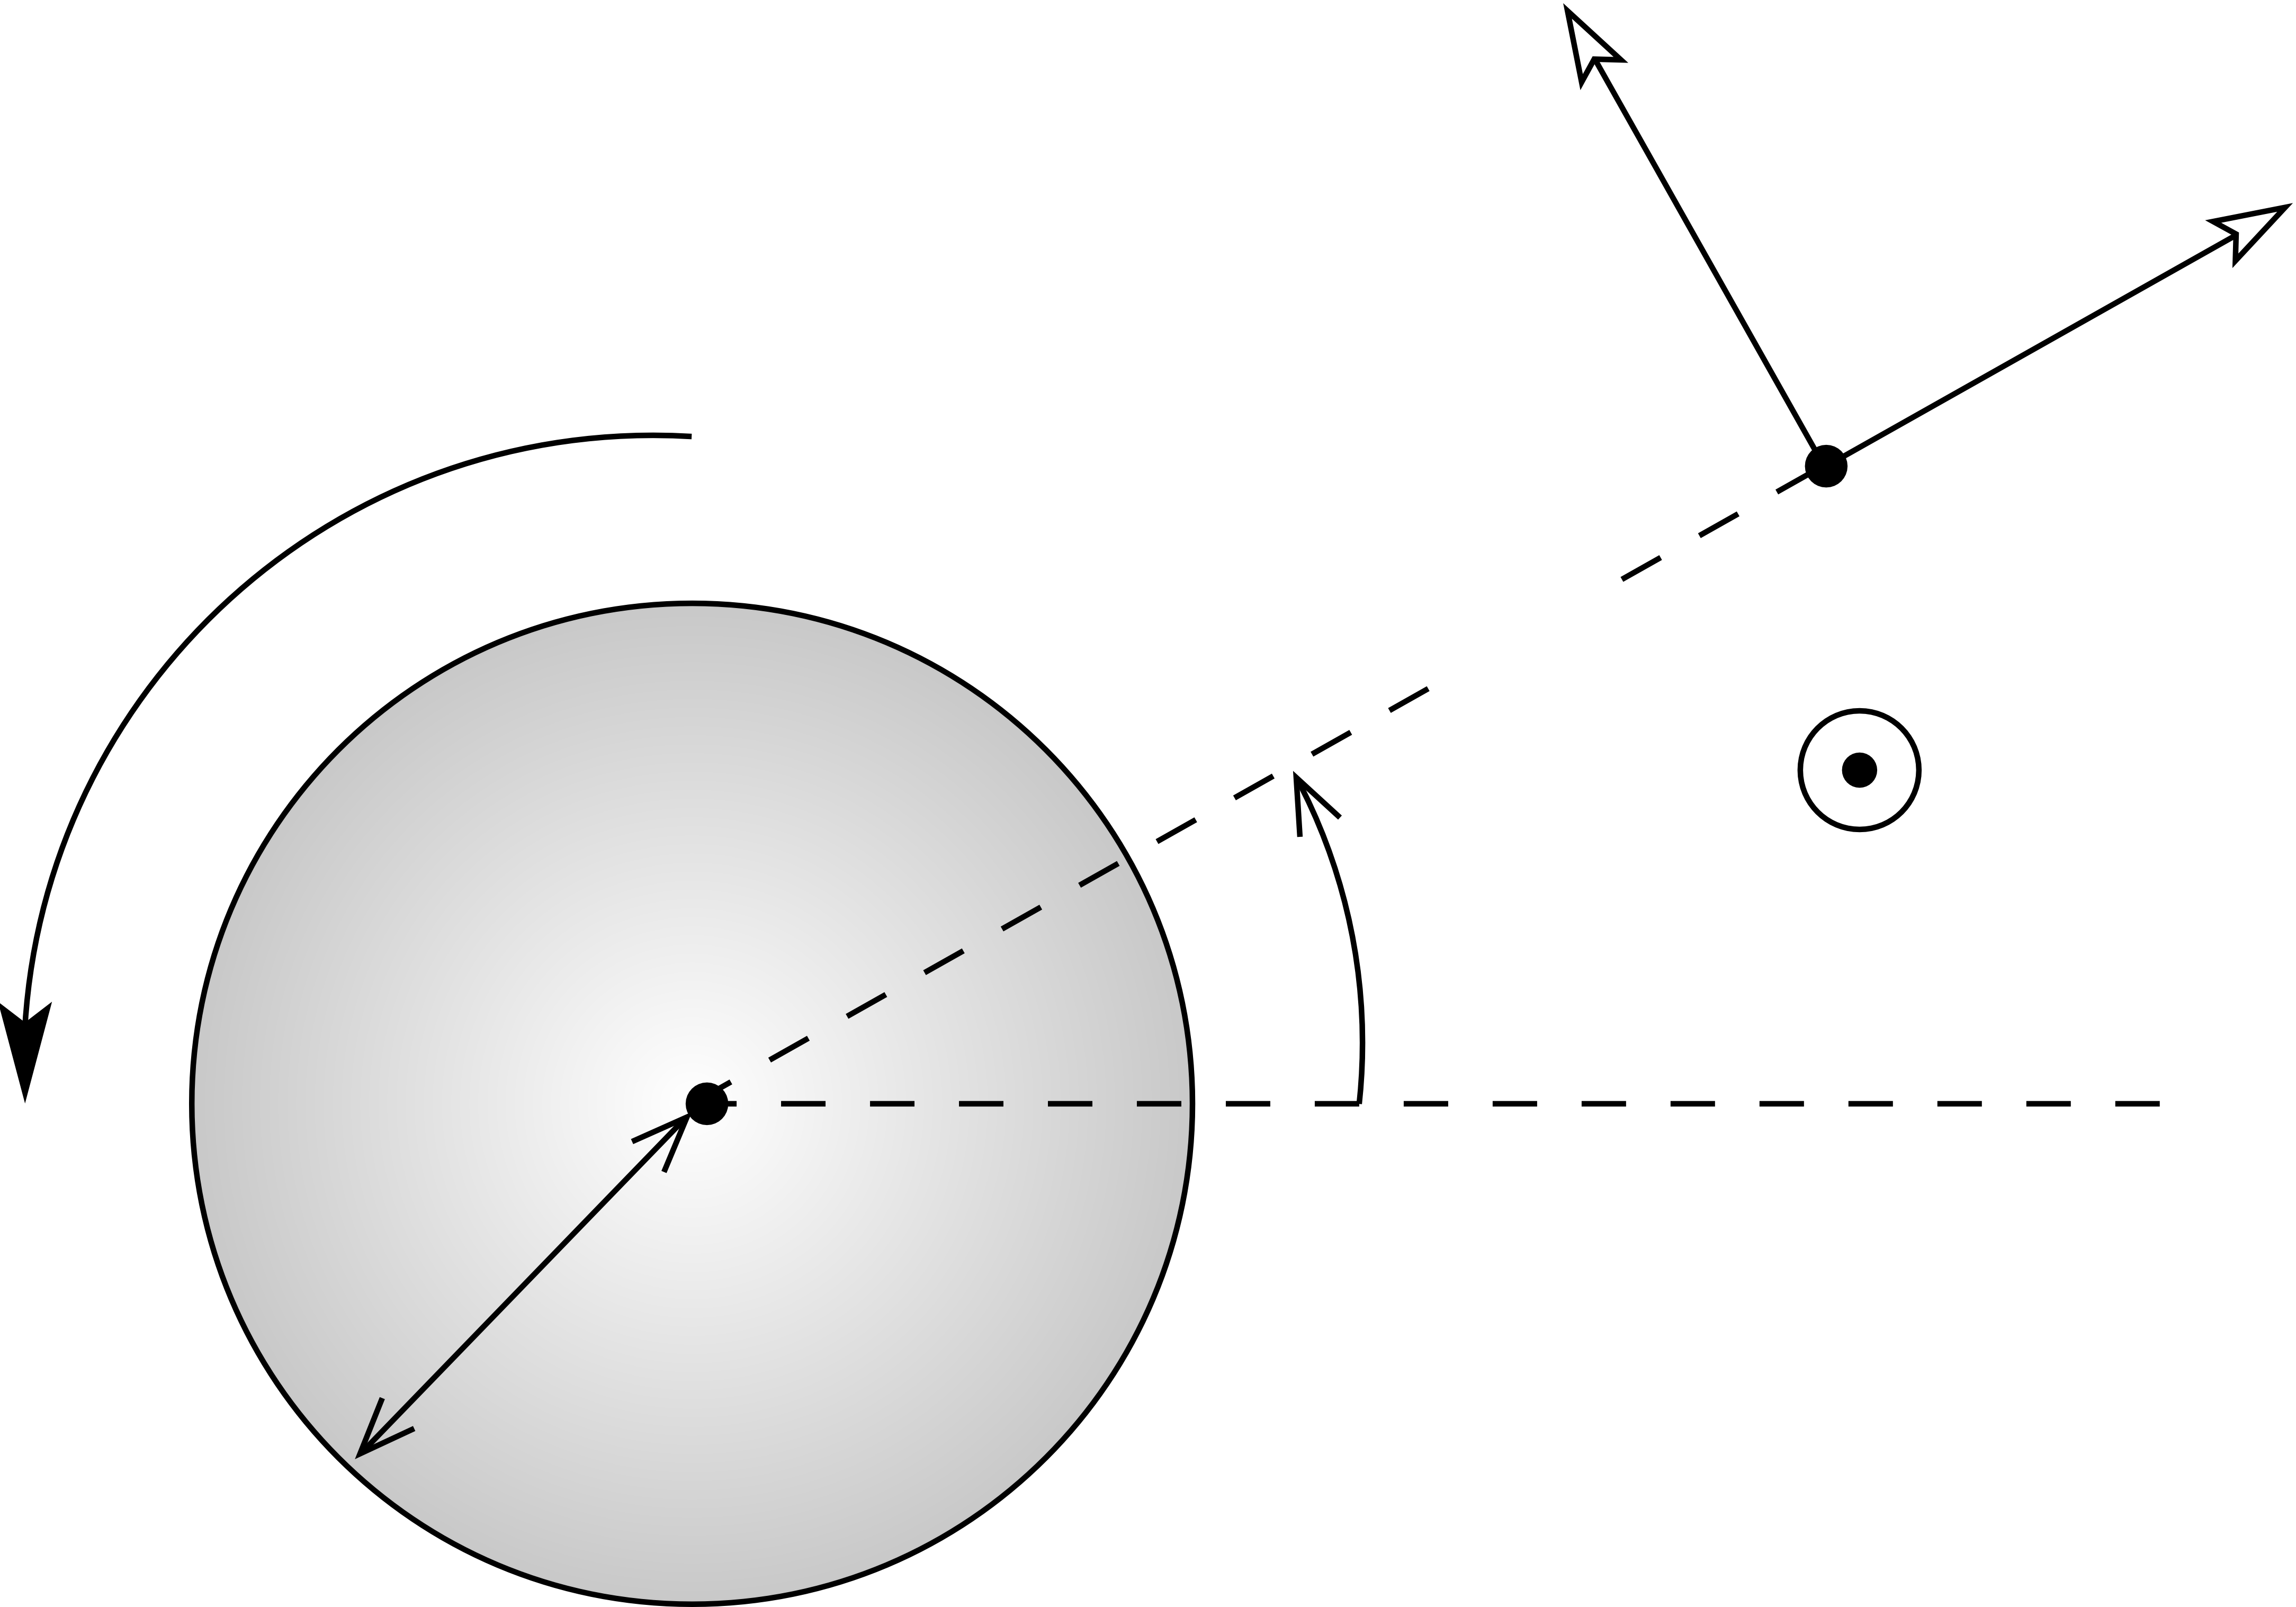
\includegraphics[width=7cm]{cylindre.png}}
\put(12, 10){$R$}
\put(5, 33){$\omega$}
\put(19, 17){$O$}
\put(43, 20){$\theta$}
\put(46, 29){$r$}
\put(67, 37){$\mathbf{e}_r$}
\put(53, 45){$\mathbf{e}_\theta$}
\put(61, 25){$\mathbf{e}_z$}
\end{picture}
\end{center}
\caption{Cylindre en rotation}
\label{fig:cylindre_tournant}
\end{figure}


Le cylindre est reli\'e \`a un moteur qui, mis en route \`a $t=0$,
lui impose une vitesse angulaire constante $\omega$ (rad/s) autour
de son axe $Oz$ (fig.~\ref{fig:cylindre_tournant}).

\begin{enumerate}
\setcounter{enumi}{0}
\item
Expliquer en quelques mots pourquoi et comment le liquide initialement
au repos va se mettre en mouvement.
On précisera en particulier le mode de transport de la quantité de mouvement
impliqué. 
Imaginer les lignes de courant de l'\'ecoulement ainsi g\'en\'er\'e
(faire un dessin).
\item
Apr\`es un r\'egime transitoire de mise en mouvement du liquide,
l'\'ecoulement tend \`a devenir stationnaire dans le voisinage du cylindre.
Quel pourrait \^etre une premi\`ere approximation de l'ordre de grandeur
de la dur\'ee $\tau$ du r\'egime transitoire ? 
\end{enumerate}
\noindent
On s'int\'eresse dor\'enavant au r\'egime quasi permanent aux temps longs $t \gg \tau$.
On rappelle que les \'equations d'un \'ecoulement incompressible plan
en coordonn\'ees polaires 
$\mathbf{u} = u(r, \theta, t) \, \mathbf{e}_r + v(r, \theta, t) \, \mathbf{e}_\theta$
s'\'ecrivent
\begin{eqnarray}
              \frac{\partial u}{\partial t}
+           u \frac{\partial u}{\partial r}
+ \frac{v}{r} \frac{\partial u}{\partial \theta} - \frac{v^2}{r}
& = &
- \frac{1}{\,\rho\,} \frac{\partial p}{\partial r} \,
+ \nu \left [ 	
\frac{\partial}{\partial r} \left (\frac{1}{r} \frac{\partial}{\partial r} (ru)  \right )  
+ \frac{1}{r^2} \frac{\partial^2 u}{\partial \theta^2} 
- \frac{2}{r^2} \frac{\partial v}{\partial \theta}
\right ]
\\
              \frac{\partial v}{\partial t}
+           u \frac{\partial v}{\partial r}
+ \frac{v}{r} \frac{\partial v}{\partial \theta} + \frac{uv}{r}
& = &
- \frac{1}{\rho r} \frac{\partial p}{\partial \theta}
+ \nu \left [ 	
\frac{\partial}{\partial r} \left (\frac{1}{r} \frac{\partial}{\partial r} (rv)  \right )  
+ \frac{1}{r^2} \frac{\partial^2 v}{\partial \theta^2} 
+ \frac{2}{r^2} \frac{\partial u}{\partial \theta}
\right ]
\\
\frac{\partial}{\partial r}(ru) + \frac{\partial v}{\partial \theta} & = & 0
\end{eqnarray}
            

\begin{enumerate}
\setcounter{enumi}{2}
\item
Justifier bri\`evement pourquoi il est a priori l\'egitime de rechercher
une solution d'\'ecoulement purement azimutal et axisym\'etrique, 
de la forme $\mathbf{u} = v(r) \, \mathbf{e}_\theta$.
\item
En injectant ce type de solution dans les \'equations du mouvement,
montrer dans un premier temps que le champ de pression ne d\'epend
que de $r$.
\item
R\'esoudre l'\'equation diff\'erentielle v\'erifi\'ee par $v(r)$
en prenant en compte les conditions aux limites d'adh\'erence \`a la paroi
imperm\'eable du cylindre en rotation et de d\'ecroissance du champ
de vitesse loin du cylindre.
\item
Montrer qu'il s'agit d'un \'ecoulement irrotationnel.
On rappelle que le rotationnel en cylindriques pour un champ bidimensionnel
$\mathbf{F} = F_r(r, \theta) \, \mathbf{e}_r + F_\theta(r, \theta) \, \mathbf{e}_\theta$
se r\'eduit \`a
\[
\textbf{rot} \, \mathbf{F} = \frac{1}{r} \left [ 
\frac{\partial}{\partial r}(rF_\theta) - \frac{\partial F_r}{\partial \theta}
\right ] \, \mathbf{e}_z
\]
\item
Calculer le champ de pression $p(r)$.
On notera $P_0$ la pression loin du cylindre.
\label{question:pression}
\end{enumerate}
\noindent
Bien que le terme visqueux $\nu \boldsymbol{\Delta} \mathbf{u}$ soit nul pour cet
\'ecoulement, ce n'est pas le cas pour les contraintes visqueuses au sein du fluide.
On rappelle que le tenseur des contraintes en coordonn\'ees polaires s'\'ecrit :
\begin{equation*}
\stackrel{\Rightarrow}{\sigma} =
\left (
\begin{array}{cc}
\sigma_{rr}      & \sigma_{r\theta} \\
\sigma_{r\theta} & \sigma_{\theta\theta}
\end{array}
\right ) 
\; \mbox{avec} \;
\sigma_{rr} = -p + 2\mu \frac{\partial u}{\partial r}, \;
\sigma_{\theta\theta} = -p + 2\mu 	\left (
	\frac{1}{r} \frac{\partial v}{\partial \theta} 
      + \frac{\partial u}{\partial r} 	\right ), \;
\sigma_{r\theta} = \mu \left (
  	\frac{1}{r} \frac{\partial u}{\partial \theta} 
      + \frac{\partial v}{\partial r}
      - \frac{v}{r}    \right )
\end{equation*}
\begin{enumerate}
\setcounter{enumi}{7}
\item
Calculer le tenseur $\stackrel{\Rightarrow}{\tau}$ des contraintes \textsl{visqueuses}.
\item
D\'eterminer la force \'el\'ementaire $d\mathbf{f}$ exerc\'ee
par le fluide sur un \'el\'ement de surface $dS$ de la paroi du cylindre.
\item
Donner l'expression du moment en $O$, not\'e $d\mathbf{M}_O$, de cette force \'el\'ementaire
puis du moment \textsl{r\'esultant} en $O$, not\'e $\mathbf{M}_O$, de la force de
frottement exerc\'ee par le fluide sur toute la surface du cylindre.
\item
En d\'eduire le couple $\mathbf{C}$ que devrait imposer le moteur au cylindre
pour maintenir la rotation \`a vitesse angulaire $\omega$ constante.
Quelle est la puissance dissip\'ee $\cal P$ ? 
\end{enumerate}

\paragraph{Questions complémentaires :}
Le liquide dans lequel est plong\'e le cylindre poss\`ede une surface libre
avec l'air ext\'erieur \`a pression atmosph\'erique $P_{atm}$.
Au repos (cylindre immobile) cette surface se trouve \`a l'altitude $z = h_0$. 
On cherche ici \`a pr\'edire comment la mise en mouvement du cylindre
va d\'eformer cette surface libre.
Le champ de vitesse d\'etermin\'e pr\'ec\'edemment n'est pas modifi\'e
et conserve la m\^eme expression $v(r)$.
Ce n'est pas le cas pour le champ de pression, qu'il faut recalculer
en notant que la d\'ependance de la pression suivant la verticale est
maintenant affect\'ee par la prise en compte de la pesanteur:
\[
\frac{\partial p}{\partial z} = -g
\]
\begin{enumerate}
\setcounter{enumi}{11}
\item
Reprendre la question~\ref{question:pression} pour calculer le champ
de pression $p(r, z)$ dans le liquide.
\item
En négligeant les effets de tension de surface, d\'eterminer 
la forme de la surface libre $z=h(r)$.
Tracer qualitativement la forme de surface libre.
\end{enumerate}

On cherche pour finir \`a d\'eterminer l'influence d'un
cylindre ext\'erieur sur le couple \`a imposer au cylindre
principal pour le maintenir \`a vitesse angulaire constante $\omega$.
On consid\`ere donc que le liquide est confin\'e entre le cylindre principal
de rayon $R$ et un second cylindre \textit{immobile} de rayon $R^\star > R$.

\begin{enumerate}
\setcounter{enumi}{13}
\item
Reprendre les questions 3 \`a 5 pour calculer le champ de vitesse $v^\star(r)$.
\item
Calculer la contrainte visqueuse exerc\'ee par le liquide sur la paroi du
cylindre principal et en d\'eduire que le moment r\'esultant en $O$ par unit\'e
de longueur du frottement visqueux sur le cylindre est de la forme
\[
\mathbf{M}_O^\star = -4\pi \mu^\star \omega R^2 \, \mathbf{e}_z
\]
o\`u $\mu^\star$ est une fonction de $\mu$, $r$ et $R^\star$ \`a d\'eterminer. 
\item
Comparer le couple qu'il faut imposer ici pour maintenir une vitesse angulaire
$\omega$ constante par rapport au cas pr\'ec\'edent o\`u le second cylindre
est absent.
\end{enumerate}








\end{document}





